\documentclass{article}

% Packages
\usepackage{amssymb,amsmath,amsthm,bbm}
\usepackage{verbatim,float,url,dsfont}
\usepackage{graphicx,subcaption,psfrag}
\usepackage{algorithm,algorithmic}
\usepackage{mathtools,enumitem}
\usepackage{multirow}
\usepackage{ragged2e}
\usepackage{xr-hyper}
\usepackage{array}

\usepackage[colorlinks=true,citecolor=blue,urlcolor=blue,linkcolor=blue]{hyperref}
\usepackage[margin=1in]{geometry}
\usepackage[round]{natbib}

\usepackage[utf8]{inputenc} % allow utf-8 input
\usepackage[T1]{fontenc}    % use 8-bit T1 fonts
\usepackage{booktabs}       % professional-quality tables
\usepackage{nicefrac}         % compact symbols for 1/2, etc.
\usepackage{microtype}      % microtypography

\ifdefined\TimesFont 
\usepackage{times} % use times font
\fi

\ifdefined\ParSkip 
\usepackage{parskip} % use par skip
\fi

% Theorems and such
\newtheorem{theorem}{Theorem}
\newtheorem{lemma}{Lemma}
\newtheorem{corollary}{Corollary}
\newtheorem{proposition}{Proposition}
\theoremstyle{definition}
\newtheorem{remark}{Remark}
\newtheorem{definition}{Definition}

% Assumption
\newtheorem*{assumption*}{\assumptionnumber}
\providecommand{\assumptionnumber}{}
\makeatletter
\newenvironment{assumption}[2]{
  \renewcommand{\assumptionnumber}{Assumption #1#2}
  \begin{assumption*}
  \protected@edef\@currentlabel{#1#2}}
{\end{assumption*}}
\makeatother

% Widebar
\makeatletter
\newcommand*\rel@kern[1]{\kern#1\dimexpr\macc@kerna}
\newcommand*\widebar[1]{%
  \begingroup
  \def\mathaccent##1##2{%
    \rel@kern{0.8}%
    \overline{\rel@kern{-0.8}\macc@nucleus\rel@kern{0.2}}%
    \rel@kern{-0.2}%
  }%
  \macc@depth\@ne
  \let\math@bgroup\@empty \let\math@egroup\macc@set@skewchar
  \mathsurround\z@ \frozen@everymath{\mathgroup\macc@group\relax}%
  \macc@set@skewchar\relax
  \let\mathaccentV\macc@nested@a
  \macc@nested@a\relax111{#1}%
  \endgroup
}
\makeatother

% Operators and shortcuts
\DeclareMathOperator*{\argmin}{argmin}
\DeclareMathOperator*{\argmax}{argmax}
\DeclareMathOperator*{\minimize}{minimize}
\DeclareMathOperator*{\maximize}{maximize}
\DeclareMathOperator*{\find}{find}
\DeclareMathOperator{\st}{subject\,\,to}

\DeclareMathOperator{\Cor}{Cor}
\DeclareMathOperator{\Cov}{Cov}
\DeclareMathOperator{\Var}{Var}
\DeclareMathOperator{\dm}{dim}
\DeclareMathOperator{\col}{col}
\DeclareMathOperator{\row}{row}
\DeclareMathOperator{\nul}{null}
\DeclareMathOperator{\rank}{rank}
\DeclareMathOperator{\nuli}{nullity}
\DeclareMathOperator{\spa}{span}
\DeclareMathOperator{\sign}{sign}
\DeclareMathOperator{\supp}{supp}
\DeclareMathOperator{\diag}{diag}
\DeclareMathOperator{\aff}{aff}
\DeclareMathOperator{\conv}{conv}
\DeclareMathOperator{\dom}{dom}
\DeclareMathOperator{\tr}{tr}
\DeclareMathOperator{\df}{df}

\def\E{\mathbb{E}}
\def\P{\mathbb{P}}
\def\R{\mathbb{R}}
\def\C{\mathbb{C}}
\def\N{\mathbb{N}}
\def\Z{\mathbb{Z}}
\def\T{\mathsf{T}}

\def\half{\frac{1}{2}}
\def\df{\mathrm{df}}
\def\hy{\hat{y}}
\def\hf{\hat{f}}
\def\hmu{\hat{\mu}}
\def\halpha{\hat{\alpha}}
\def\hbeta{\hat{\beta}}
\def\htheta{\hat{\theta}}
\def\indep{\perp\!\!\!\perp}
\def\th{^{\textnormal{th}}}

\def\cA{\mathcal{A}}
\def\cB{\mathcal{B}}
\def\cD{\mathcal{D}}
\def\cE{\mathcal{E}}
\def\cF{\mathcal{F}}
\def\cG{\mathcal{G}}
\def\cK{\mathcal{K}}
\def\cH{\mathcal{H}}
\def\cI{\mathcal{I}}
\def\cL{\mathcal{L}}
\def\cM{\mathcal{M}}
\def\cN{\mathcal{N}}
\def\cP{\mathcal{P}}
\def\cS{\mathcal{S}}
\def\cT{\mathcal{T}}
\def\cW{\mathcal{W}}
\def\cX{\mathcal{X}}
\def\cY{\mathcal{Y}}
\def\cZ{\mathcal{Z}}

\usepackage{adjustbox}
\renewcommand{\hat}{\widehat} % DJM: I find the regular hat hard to see
\newcommand{\given}{\, \vert \,}
\DeclareMathOperator{\bias}{Bias}

\usepackage{xcolor}
\newcommand{\ahcomment}[1]{{\color{red}[AH: #1]}}
\newcommand{\rjtcomment}[1]{{\color{purple}[RJT: #1]}}
\newcommand{\djmcomment}[1]{{\color{teal}[DJM: #1]}}
\newcommand{\jmgcomment}[1]{{\color{cyan}[JMG: #1]}}

\title{Challenges in Estimating Time-Varying Epidemic Severity Rates from
  Aggregate Data} 

\author{Jeremy Goldwasser\thanks{Department of Statistics, University of
    California, Berkeley} 
  \and  
  Addison J.\ Hu\thanks{Department of Statistics, Carnegie Mellon University}
  \and 
  Alyssa Bilinski\thanks{Departments of Health Policy and Biostatistics, Brown University} 
  \and
  Daniel J.\ McDonald\thanks{Department of Statistics, University of British
    Columbia} 
  \and 
  Ryan J.\ Tibshirani\footnotemark[1]}

\date{}

\begin{document}
\maketitle

\begin{abstract}
Severity rates like the case-fatality rate and infection-fatality rate are
key metrics in public health. To guide decision-making in response to changes
like new variants or vaccines, it is imperative to understand how these rates
shift in real time. In practice, time-varying severity rates are typically
estimated using a ratio of aggregate counts. We demonstrate that these
estimators are capable of exhibiting large statistical biases, with concerning
implications for public health practice, as they may fail to detect heightened 
risks or falsely signal nonexistent surges. We supplement our mathematical 
analyses with experimental results on real and simulated COVID-19 data. Finally,
we briefly discuss strategies to mitigate this bias, drawing connections with
effective reproduction number ($R_t$) estimation.    
\end{abstract}

\section{Introduction}

Several public health metrics of interest express the probability that a second,
often more serious outcome will follow a primary event. For example, the
case-fatality rate (CFR) and infection-fatality rate (IFR) are commonly used to
assess the deadliness of an epidemic \citep{nishiuraEx1, nishiuraEx2,
  cfr_line_list, timevar_ifr, lancet_ifr}. Another central example of a
``severity rate'', which is a term that we use for metrics of this general form,
is the hospitalization-fatality rate (HFR) \citep{HFR_linelist3, HFR_linelist1,  
  HFR_linelist2}.

In an ideal setting, severity rates can be obtained directly from a
comprehensive line-list or claims data set containing individual patient
outcomes \citep{HFR_linelist3, cfr_line_list, HFR_linelist1, HFR_linelist2}.
However, in fast-moving epidemics like COVID-19, large-scale tracking of
individuals has been infeasible, especially in real time. Instead, severity
rates are routinely estimated from aggregate count data. While it is common to
assume they are constant in time \citep{ghani, jewell2007nonparametric,
  reich2012estimating, lancet_controversial}, consequential shifts in severity
rates can occur in response to factors such as new therapeutics, vaccines, and
variants \citep{nyt}. Time-varying severity rates are often estimated with a
ratio of primary and secondary aggregate data streams. For example, aggregate 
case and death counts were widely used to estimate and report COVID-19 CFRs, 
both in the academic literature \citep{yuan2020monitoring, timevar_ifr,
  horita2022global, LIU2023100350, germany} and also in major news outlets like
The Atlantic \citep{atlantic} and The Wall Street Journal \citep{wsj}. In fact,
ratio estimators are so common that CFR is often (mis)labeled the case-fatality
\emph{ratio}. 

In this work, we show that these ratio estimators are prone to nontrivial
statistical bias. Bias arises as a consequence of changing severity
rates---precisely when time-varying estimates should be most useful. It also 
arises due to misspecification of the delay distribution, which relates events, 
like cases and deaths in CFR. This is particularly troublesome for the popular
lagged ratio estimator, which divides values of two aggregate data streams. We
validate these findings empirically, tracking the hospitalization-fatality rate
(HFR) during COVID-19. The ratio estimators failed to quickly signal increased
risk in the onset of the Delta wave; later, in the aftermath of the inital
Omicron wave, they surged while the true HFR fell. We provide heuristics for
when to expect this bias in practice, and discuss ideas for alternative
methodology which may avoid it. 

\section{Methods}
\label{sec:methods}

In this section, we introduce the main estimators we study, and analyze their 
bias. Subsequently, we detail the data used for empirical study and validation. 

\subsection{Severity rate estimators}
\label{sec:defs}

Severity rates convey the probability that a primary event will result in a
secondary event in the future. In the case of CFR, for example, a primary event
is a positive COVID-19 case and a secondary event is a death with a positive
test result. Formally, a time-varying severity rate at time $t$ is generally
defined as:  
\begin{equation}
\label{eq:severity}
p_t = \P(\text{secondary event will occur} \given \text{primary event at time 
  $t$}).   
\end{equation}
Here, $t$ may represent a discrete interval of time, such as a given day or 
week. It also may be understood in a continuous-time fashion. Although this will    
not be our focus in this paper, the same general principles apply in the
continuous-time case. For simplicity, we will consider only the discrete-time 
setting, and we index time steps via integers, as in $t=0,1,2,\dots$.    

Throughout, we denote by $\{X_t\}$ and $\{Y_t\}$ the aggregate time series of 
new primary and secondary events, respectively. These are often counts, and we
will generally refer to them as such. At time $t$, we assume data for all past
$s \leq t$ is available, but future data is not. Therefore real-time estimates of
$p_t$ can only rely on past counts \smash{$\{X_s\}_{s\leq t}$} and
\smash{$\{Y_s\}_{s\leq t}$}. In practice, to stabilize estimates, smoothed
counts are often used in place of raw counts. This may be simply absorbed into 
the notation for $X_t$ and $Y_t$, and we do not address smoothing explicitly in
the formulation of the estimators, but refer back to this issue in Section
\ref{sec:setup}.  

\paragraph{Lagged estimator.} 

The canonical estimator for time-varying severity rates is a ratio between
the counts of primary and secondary events, offset by a lag $\ell$. This
estimator is widely-used in epidemiology, both in the academic literature and in 
public health practice and communication (e.g., \citealp{wsj, atlantic,
  yuan2020monitoring, timevar_ifr, thomas2021estimating, horita2022global,
  LIU2023100350, germany}). For concreteness, we define the \emph{lagged ratio} 
at time $t$ as:   
\begin{equation}
\label{eq:lagged}
\hat{p}_t^\ell = \frac{Y_t}{X_{t-\ell}},
\end{equation}
where $\ell \geq 0$ is a given parameter (often chosen to maximize
cross-correlation between $\{X_t\}$ and $\{Y_t\}$).      

\paragraph{Convolutional estimator.} 

Alternative methods for estimating severity rates utilize a delay distribution,
which relates the two time series. The delay distribution at time $t$ and lag
$k$ is defined as: 
\[
\pi_k^{(t)} = \P(\text{secondary event at $t+k$} \given \text{primary event at
  $t$, secondary event occurs}).  
\]
Throughout, we assume that the delay distribution has a finite support
of $d$ time steps. We also assume the delay distribution is stationary:
\smash{$\pi_k^{(t)} = \pi_k$} for all $k$ and $t$. (In reality, delay
distributions may themselves be time-varying, and this creates its own set of
challenges, which only exacerbate the ones we highlight in this paper for a
fixed delay distribution.) While the delay distribution is generally unknown,
several tools exist to estimate them from aggregate or line-list data (see
\citealp{delay_distrs} for a nice review). Given $\pi$, we can express the
expected number of secondary events at time $t$ as follows: 
\begin{align}
\E[Y_t \given \{X_s\}_{s\leq t}]
&= \sum_{k=0}^d X_{t-k} \P(\text{secondary at $t$} \given \text{primary at
  $t-k$}) \nonumber \\   
&= \sum_{k=0}^d X_{t-k} \P(\text{secondary after $k$ time steps} \given
  \text{secondary occurs, primary at $t-k$}) \nonumber \\
&\hspace{200pt} \times\P(\text{secondary occurs} \given\text{primary at $t-k$})
  \nonumber \\  
\label{eq:model}
&= \sum_{k=0}^d X_{t-k} \pi_k p_{t-k}.
\end{align}
This is a convolution of the delay distribution against the product of primary
incidence and the severity rate. If the severity rate remains constant, $p_{t-k}
= p_t$ for all $k$ between $0$ and $d$, then the expression in \eqref{eq:model}
simplifies to \smash{$\E[Y_t \given \{X_s\}_{s\leq t}] = p_t \sum_{k=0}^d
  X_{t-k} \pi_k$}. As studied in \citet{UKpaper}, we can rearrange this
relationship in order to estimate the severity rate at $t$, after plugging-in an
estimate $\gamma$ of the delay distribution $\pi$:   
\begin{equation}
\label{eq:conv}
\hat{p}_t^\gamma = \frac{Y_t}{\sum_{k=0}^d X_{t-k} \gamma_k}.
\end{equation}
We call this the \emph{convolutional ratio} estimator of the severity rate; in
the notation here, the superscript in \smash{$\hat{p}_t^\gamma$} emphasizes that
$\gamma$ is the distribution used in the definition of the estimator
\eqref{eq:conv}. To reiterate, in moving from \eqref{eq:model} to
\eqref{eq:conv}, we are implicitly assuming that the severity rate $p_t$ is
constant over the interval of time from $t-d$ and $t$. Of course, this runs in
contradiction to the fact that we are trying to estimate a time-varying severity
rate in the first place. As we will see shortly, this can create significant
bias in the convolutional ratio.  

Some further comments are in order. The convolutional ratio has a longer history
of study and use in the literature on estimating stationary severity
rates. Indeed, \citet{nishiura} developed the estimator in this setting,  
and used it to analyze the CFR in the H1N1 influenza pandemic of 2009. (The only 
difference to \eqref{eq:conv} is that in the stationary case we aggregate both
the numerator and denominator over all past data.) This estimator, which is
sometimes called the \emph{delay-adjusted} estimator of the severity rate, is
popular in the academic literature and public health practice (e.g., 
\citealp{nishiuraEx1, nishiuraEx2, Russell2020, Unnikrishnan2021}), though   
arguably less popular than the lagged ratio. The package \texttt{cfr}
\citep{cfr_package} gives an R implementation, for both the stationary and
time-varying cases.  

Furthermore, we note that \eqref{eq:conv} can be seen as a generalization of the  
lagged ratio estimator \eqref{eq:lagged}: when we take $\gamma$ to be a point
mass at lag $\ell$, i.e., $\gamma_\ell = 1$ and $\gamma_k = 0$ for all $k \not=
\ell$, then \eqref{eq:conv} reduces to \eqref{eq:lagged}.   

\paragraph{Connection with reproduction numbers.} 

Severity rates bear a natural connection with reproduction numbers. Both the
true severity rate as defined in \eqref{eq:severity} and the case reproduction
number $R_t$ are defined as the average number of secondary events produced by a
single primary event at $t$, but in contrast to severity rates, reproduction
numbers have infections as the primary and secondary events, where a single
infection can produce more than one follow-on infection. Playing the role of the
delay distribution $\pi$ in our setting is the generation interval distribution
in reproduction numbers, which measures the time in between primary and
secondary infections.  

Severity rates and reproduction numbers can also be estimated similarly. Because
primary events at $t$ produce secondary events after $t$, their effect is not
observed in real time. Therefore, standard real-time estimators for severity
rates \eqref{eq:lagged}, \eqref{eq:conv} and for $R_t$ both analyze the number
of  secondary events at $t$ produced by relevant primary events. In words, this 
adopts a ``backward-looking'' perspective (possible in real time), rather the 
the ``forward-looking'' perspective inherent to the definition in
\eqref{eq:severity}. 

For reproduction numbers, the backward-looking quantity has its own name:
\emph{instantaneous} $R_t$, which is the average number of secondary infections
at time $t$ produced by a single primary infection in the past. One of the most
popular traditional estimators of instantaneous $R_t$ is based on an essentially 
identical idea to the convolutional ratio \citep{fraser2007, wallinga2007how}: 
\begin{equation}
\label{eq:instRt}
\hat{R}_t = \frac{I_t}{\sum_{k=1}^d I_{t-k} g_k}.
\end{equation}
Here, $I_t$ denotes the number of new infections at $t$, and $g$ is the
generation interval distribution. Note that the difference between
\eqref{eq:conv} and \eqref{eq:instRt} is that the latter uses the same aggregate 
time series, infections, in both the numerator and denominator. While more
modern frameworks for estimating instantaneous $R_t$ are often Bayesian (e.g.,
\citealp{cori2013new}), the underlying basic point estimates are still the same.
% By contrast, the popular estimator from \citet{wallinga_teunis} is analogous
% to equation \eqref{eq:severity}, but requires data after time $t$.    

\subsection{Well-specified analysis}
\label{sec:wellspecified}

First we analyze the bias of the convolutional ratio \eqref{eq:conv} in what we  
call the \emph{well-specified} case, where the true delay distribution $\pi$ is 
known. Formally, for an estimator \smash{$\hat{p}_t$} of $p_t$, we define its
bias as:     
\[
\bias(\hat{p}_t) = \E[\hat{p}_t \given \{X_s\}_{s\leq t}] - p_t. 
\]

\begin{proposition}
\label{prop:OracleBias}
The bias of the convolutional ratio \smash{$\hat{p}_t^\pi$} (where the true
delay distribution $\pi$ is known) is 
\begin{equation}
\label{eq:OracleBias}
\bias(\hat{p}_t^\pi)  = \sum_{k=0}^d \Bigg[ \frac{X_{t-k}\pi_k}{\sum_{j=0}^d
  X_{t-j}\pi_j} (p_{t-k}-p_t) \Bigg]. 
\end{equation}
\end{proposition}
The proof of Proposition \ref{prop:OracleBias} is elementary and given in
Appendix \ref{apx:OracleBias}. The bias \eqref{eq:OracleBias} of the
convolutional ratio estimator of the severity rate depends on three factors,
which we discuss next. Figure \ref{fig:wellspecified} provides an accompanying
illustration.     

\begin{enumerate}
\item \textbf{Changes in severity rate}. The central component of this bias
  expression is the difference $p_{t-k}-p_t$. When the severity rate is constant
  over the $d$ preceding time points, the convolutional ratio is unbiased 
  (because this difference is zero). This falls in line with the motivation used
  to derive this estimator, as explained in the last subsection. But when 
  severity rates change before $t$, these difference terms will be nonzero, in
  which case the estimator will be generally biased. %\footnote{It is possible
   %that this estimator could still be unbiased in the unlikely event that
   %individual components in the summation over $k$ exactly cancel each other.}   
  Figure \ref{fig:toy_hfr} shows a simple example of this: the estimated
  severity rates are most inaccurate in periods where the true rate is changing
  quickly.        

  To make matters worse, the bias is in the opposite direction of the trend we 
  want to detect; for example, suppose the severity rate is monotonically
  falling, with $p_t < p_{t-1} < \dots < p_{t-d}$. The bias will then be
  positive, meaning the ratio estimates do not decline with the true rate. In
  fact, the estimated severity may even rise, not fall. Conversely, when true
  severity rates are rising, the estimates will be too low. 

\item \textbf{The delay distribution}. How much the changing severity rates
  impact the bias depends on the shape of the delay distribution $\pi$. In
  general, the bias will be greatest when the delay distribution has a long
  enough tail to upweight significant differences in severity rate. While this
  distinction may appear subtle, Section \ref{sec:results} highlights its
  surprisingly large effects. The simple example in Figure \ref{fig:toy_delay}
  also shows significant differences in bias between shorter and longer delay
  distributions.     

\item \textbf{The primary incidence curve.} Changing primary incidence $X_t$ 
  will also affect the bias, presuming the severity rate changes roughly 
  monotonically in the recent past. Intuitively, this up- or down-weights the
  terms $X_{t-k}\pi_k (p_{t-k} - p_t)$ at times further from the present, which  
  are likely to contribute the most bias. In general, falling primary incidences
  will amplify the bias, whereas rising events will minimize it. Figure
  \ref{fig:toy_primary} provides an illustration of this phenomenon.   
\end{enumerate}

\begin{figure}[htb]
\centering
\begin{subfigure}[b]{0.325\linewidth}
  \centering
  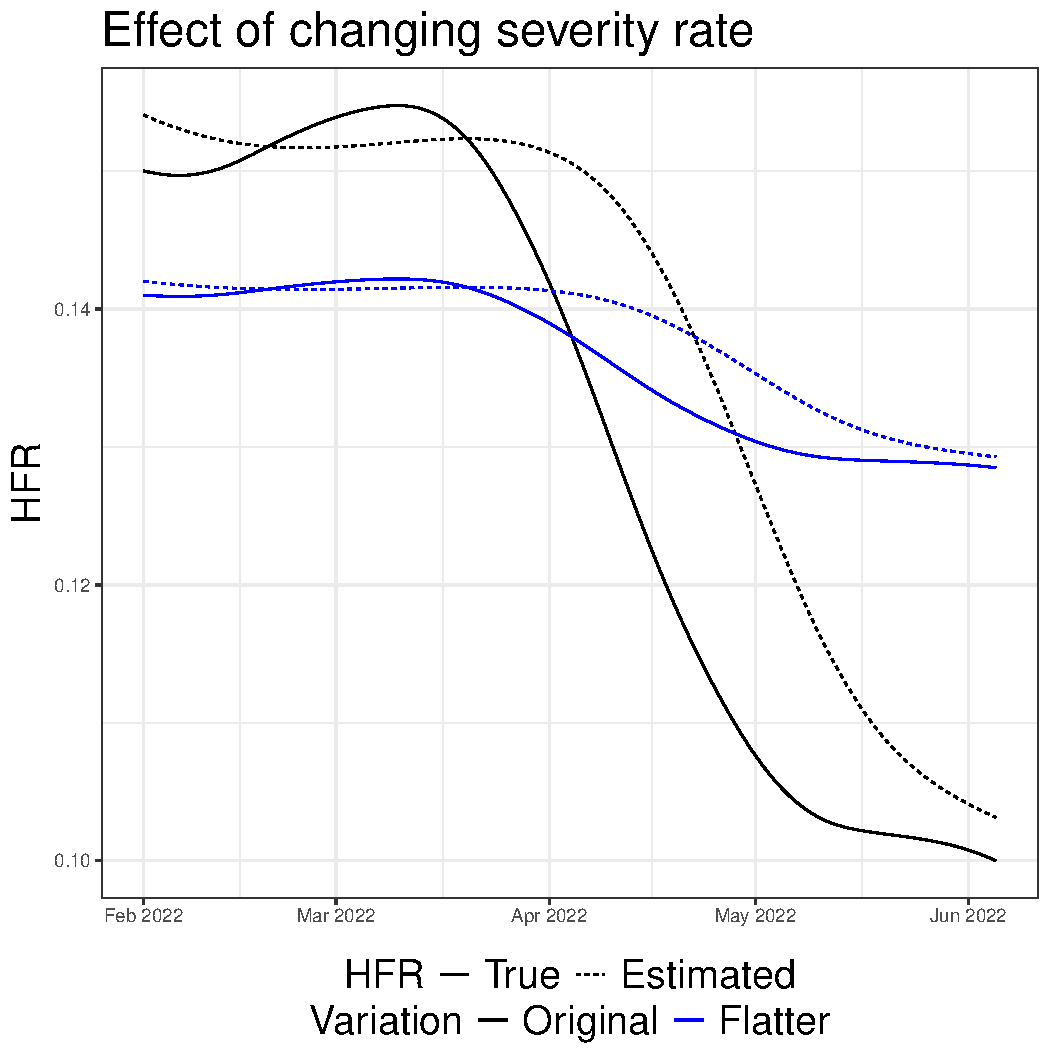
\includegraphics[width=\linewidth]{Figures/Simulated/toy_chging_hfr.pdf} 
  \caption{}
  \label{fig:toy_hfr}
\end{subfigure}
\begin{subfigure}[b]{0.325\linewidth}
  \centering
  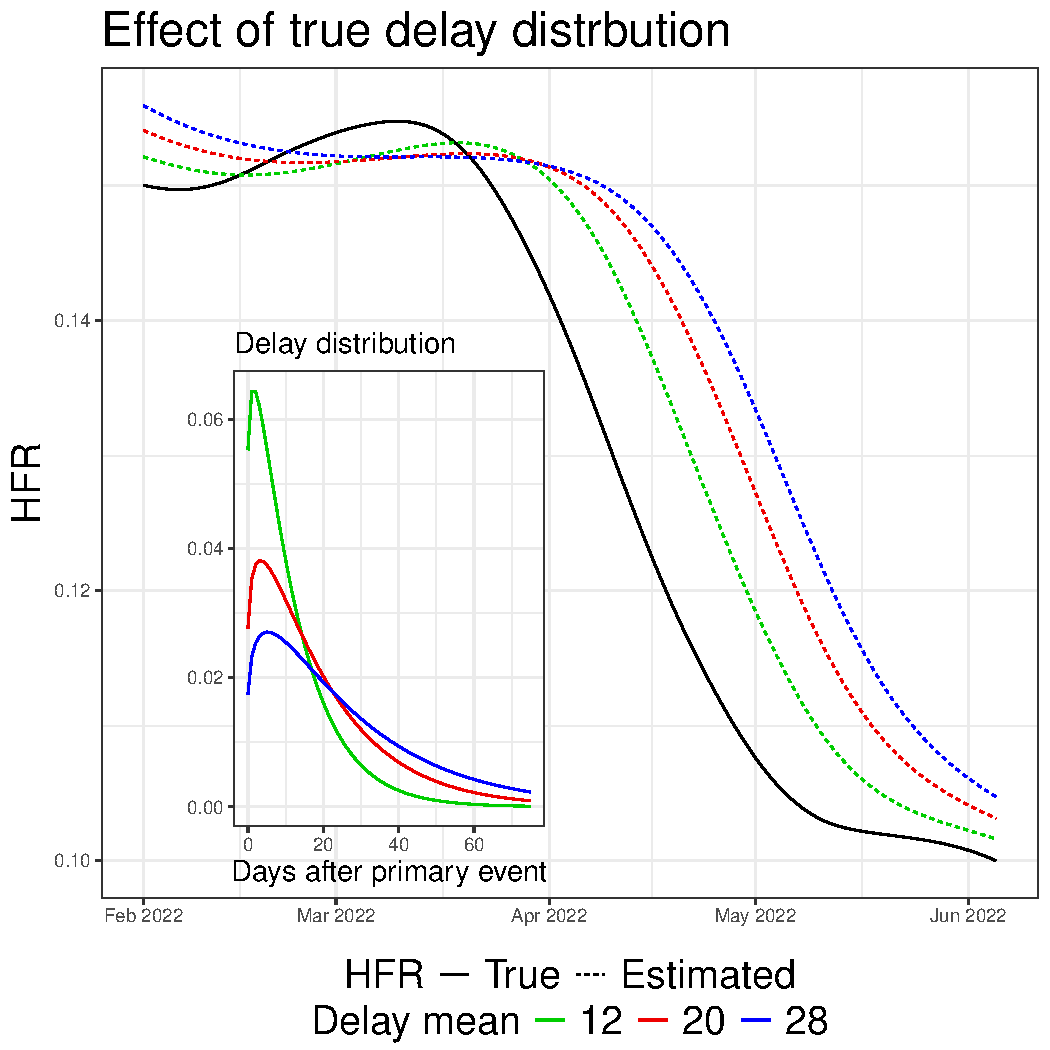
\includegraphics[width=\linewidth]{Figures/Simulated/toy_delay_distr.pdf}
  \caption{}
  \label{fig:toy_delay}
\end{subfigure}
\begin{subfigure}[b]{0.325\linewidth}
  \centering
  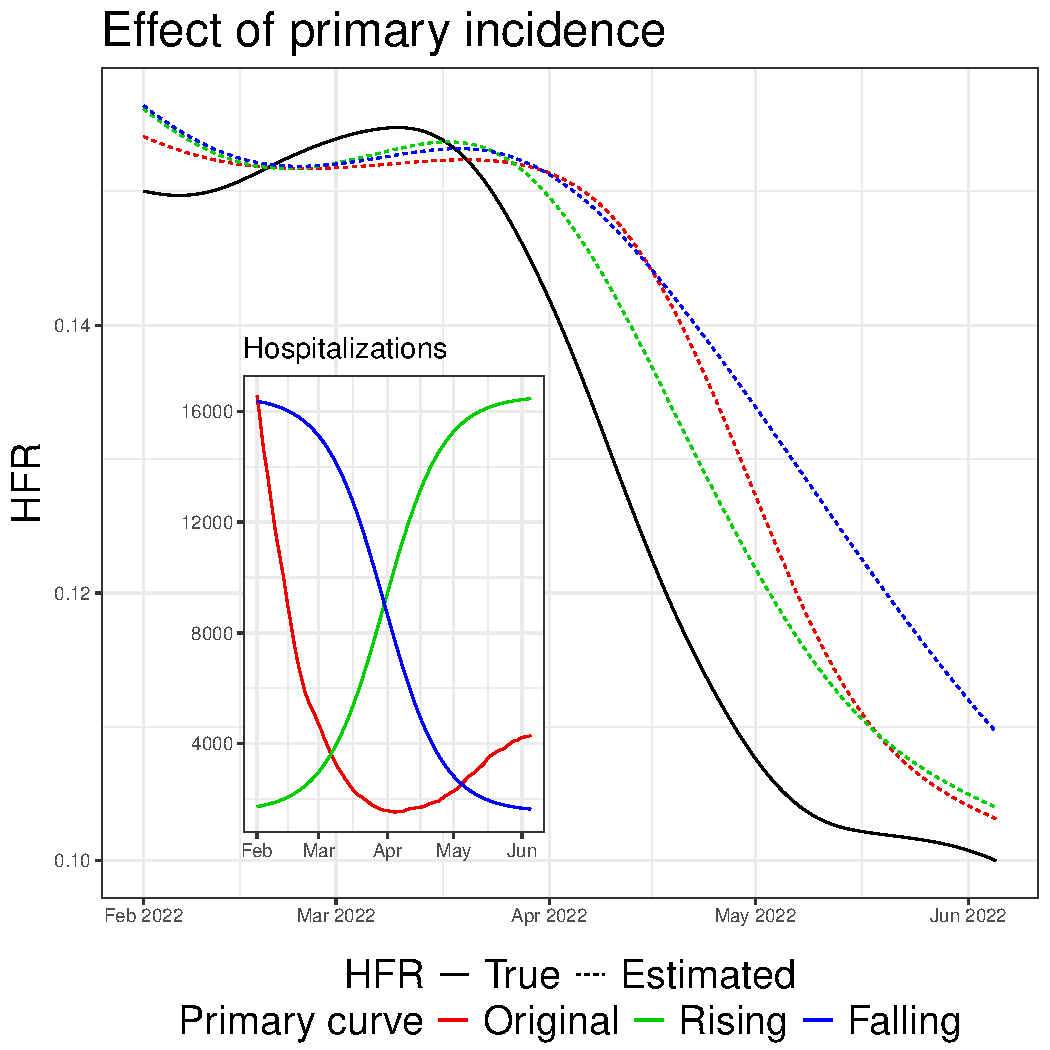
\includegraphics[width=\linewidth]{Figures/Simulated/toy_chging_primary.pdf} 
  \caption{}
  \label{fig:toy_primary}
\end{subfigure}
\caption{Simple examples which illustrate the effects of the three factors
  explained above on the bias \eqref{eq:OracleBias} in estimating the severity
  rate. The primary incidence curve measures COVID-19 hospital admissions, as
  reported to the HHS in early 2022. We then simulate a secondary incidence
  curve, COVID-19 deaths, from \eqref{eq:model}, without noise. The underlying  
  HFR curve $p_t$ and delay distribution $\pi$ used (in simulating deaths) were 
  derived from external data sources, as explained in more detail in Section
  \ref{sec:setup}.}      
\label{fig:wellspecified}
\end{figure}
      
Appendix \ref{apx:analysis} provides further analysis, by discussing 
simplified settings in which the bias \eqref{eq:OracleBias} described in
Proposition \ref{prop:OracleBias} itself simplifies in elucidating ways.   

\subsection{Misspecified analysis}
\label{sec:misspecified}

We now analyze the bias of the convolutional ratio \eqref{eq:conv} for an
arbitrary distribution $\gamma$. Recall that $\pi$ denotes the true delay
distribution in \eqref{eq:model}. We refer to the present as the
\emph{misspecified} case, as $\gamma$ may differ from $\pi$.    

\begin{proposition}
\label{prop:MispBias}
The bias of the convolutional ratio \smash{$\hat{p}_t^\gamma$} (where the true 
delay distribution $\pi$ is unknown, and the working delay distribution $\gamma$
is arbitrary, but also supported on $d$ time steps) is
\begin{equation}
\label{eq:MispBias}
\bias(\hat{p}_t^\gamma) = A_t^\gamma \bias(\hat{p}_t^\pi) + p_t (A_t^\gamma-1),  
\end{equation}
where \smash{$A_t^\gamma = \sum_{j=0}^d X_{t-j}\pi_j \,\big/\, \sum_{j=0}^d 
  X_{t-j} \gamma_j$}. This compares how the delay distributions convolve against  
the most recent primary incidence levels. 
\end{proposition}

The proof of Proposition \ref{prop:MispBias} is again elementary, and given in 
Appendix \ref{apx:MispBias}. Under misspecification, the proposition gives an
additive decomposition \eqref{eq:MispBias} of the convolutional ratio bias,
based on the well-specified bias \smash{$\bias(\hat{p}_t^\pi)$} (as studied in
Proposition \ref{prop:OracleBias}), and a misspecification factor
\smash{$A_t^\gamma$}. At the outset, we note that if $\pi = \gamma$ (no  
misspecification), we have \smash{$A_t^\gamma = 1$}, and \eqref{eq:MispBias}
reduces to the well-specified bias. Generally, values of \smash{$A_t^\gamma >
  1$} amplify the oracle bias and add positive misspecification bias \smash{$p_t
  (A_t^\gamma-1) > 0$}; meanwhile, values of \smash{$A_t^\gamma < 1$} shrink the
oracle bias and add negative misspecification bias \smash{$p_t (A_t^\gamma-1) <
  0$}. 

Whether or not misspecification contributes a larger magnitude of bias overall
hence depends on whether or not the sign of the misspecification term \smash{$p_t 
  (A_t^\gamma-1)$} agrees with the sign of the oracle bias
\smash{$\bias(\hat{p}_t^\pi)$}. This need not always be the case, though in our
experience, it is often true in both real and simulated experiments, as we will
see in Section \ref{sec:results}. Here, to gain more insight, we study the
behavior of the bias in three settings: 
\begin{enumerate} 
\item Smooth $\gamma$ with a lighter tail and smaller mean than $\pi$ (more mass
  concentrated at recent time points).    
\item Smooth $\gamma$ with a heavier tail and larger mean than $\pi$ (less mass
  concentrated at recent time points).    
\item Nonsmooth $\gamma$, with a point mass at lag $\ell$; we reiterate that in 
  this case the convolutional ratio reduces to the lagged ratio
  \smash{$\hat{p}_t^\ell$} in \eqref{eq:lagged}. We also note that its
  misspecification factor \smash{$A_t^\gamma$} reduces to a quantity we
  similarly denote \smash{$A_t^\ell = \sum_{j=0}^d X_{t-j}\pi_j \,\big/\,
    X_{t-\ell}$}, and its bias \eqref{eq:MispBias} reduces to: 
  \begin{equation}
  \label{eq:LagBias}
  \bias(\hat{p}_t^\ell) = \frac{\sum_{j=0}^d X_{t-j}\pi_j}{X_{t-\ell}}
  \bias(\hat{p}_t^\pi) + p_t \Bigg(\frac{\sum_{k=0}^d X_{t-k}\pi_k}{X_{t-\ell}}
  - 1 \Bigg).  
\end{equation}
\end{enumerate}

We discuss the behavior of the bias in these three settings, as a function of
the primary incidence curve (which drives bias through the misspecification
factor \smash{$A_t^\gamma$}). Figure \ref{fig:misspecified} provides an
accompanying illustration.

\paragraph{Primary incidence rising.} 

Consider the case where primary events are rising---first slowly, then rapidly
before leveling off. A lighter-tailed $\gamma$ will place more weight
on recent time points, with higher counts, than $\pi$; thus \smash{$\sum_{j=0}^d  
  X_{t-j}\gamma_j > \sum_{j=0}^d X_{t-j}\pi_j$}, so \smash{$A_t^\gamma <
  1$}. The opposite occurs for a heavier-tailed $\gamma$: this
places more weight on distant low-count time points and less on the ongoing
surge, so \smash{$A_t^\gamma > 1$}. A point mass distribution $\gamma$ places
all of its mass on $X_{t-\ell}$, and during the steepest phase of the rise, this
is considerably less than $X_t$. The true delay $\pi$ distributes mass across
the  $d$ most recent time points, and a large fraction of its mass will be
convolved against the last $\ell-1$ time points, whose counts exceed
$X_{t-\ell}$. The times before $t-\ell$ have less of an offsetting effect, 
because incidence has risen at a  growing rate. Hence, during a surge we will 
see \smash{$X_{t-\ell} < \sum_{j=0}^d X_{t-j}\pi_j$}, and \smash{$A_t^\ell >
  1$}. However, the behavior of \smash{$A_t^\ell$} will be generally more
erratic than \smash{$A_t^\gamma$} for a smooth distribution $\gamma$, as the
denominator in the former is less smooth as $t$ varies. 

Figure \ref{fig:misspecified} visualizes this as hopitalizations (primary
events) rise between December 2021 and mid-January 2022. Throughout this period
\smash{$A_t^\gamma$} is below/above 1 for the light-tailed/heavy-tailed
$\gamma$. Meanwhile, \smash{$A_t^\ell$} spikes to 1.25 in early January.  
Correspondly, the lagged HFR rises to 20\% when the true one drops to 15\%.    

\begin{figure}[p]
\centering
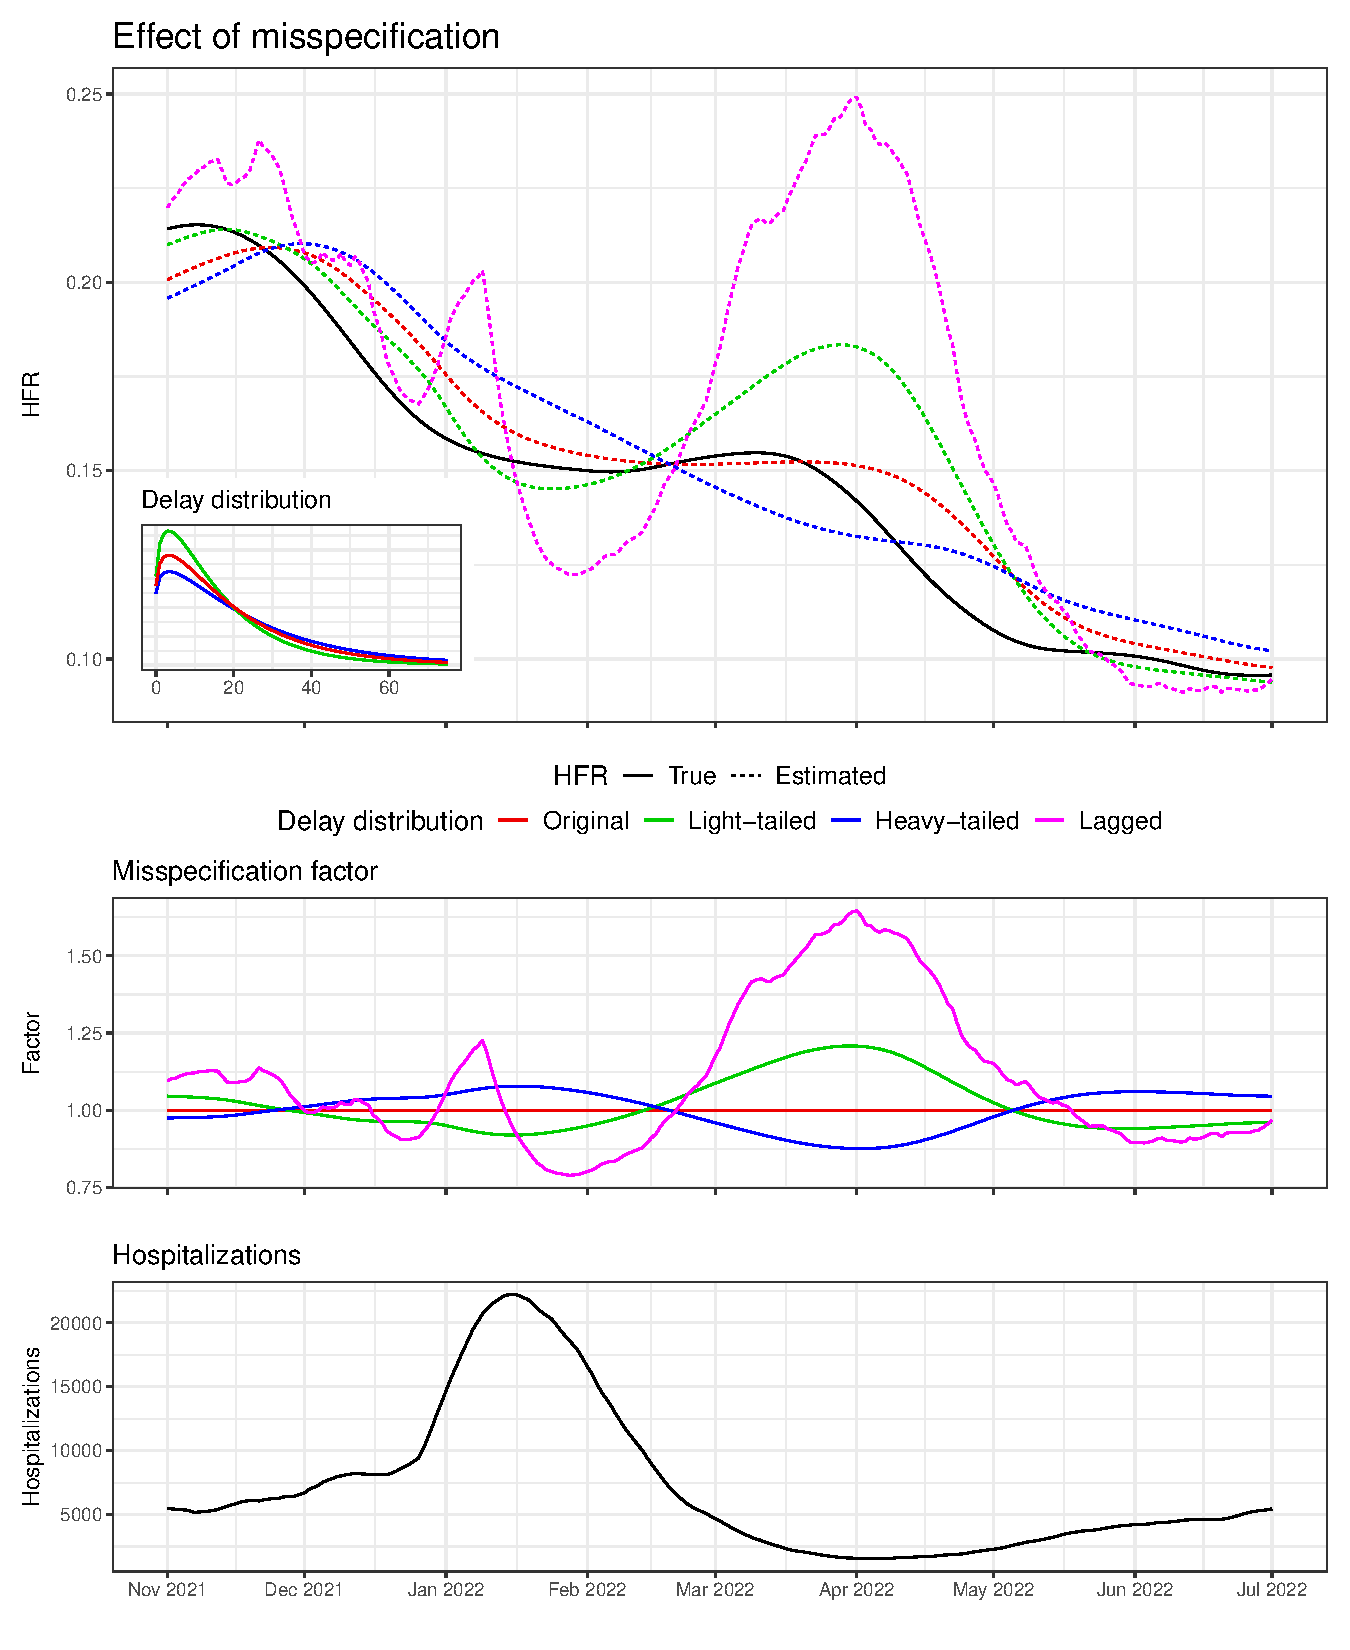
\includegraphics[width=0.9\linewidth]{Figures/Simulated/toy_misp.pdf}
\caption{Examples of convolutional ratio estimates under misspecification of the
  delay distribution.
  As in Figure \ref{fig:wellspecified}, the primary events are COVID-19
  hospitalizations, as reported to the HHS, and secondary events are deaths 
  simulated noiselessly from \eqref{eq:model}. The underlying HFR curve $p_t$
  and delay distribution $\pi$ used in the simulation were fit using external
  data sources detailed shortly in Section \ref{sec:setup}. The lagged ratio
  estimator used $\ell=16$, chosen to maximize cross-correlation (between
  hospitalizations and deaths).} 
\label{fig:misspecified}
\end{figure}

\paragraph{Primary incidence falling.}

Next assume primary incidence reaches a maximum and begins to fall. The smooth
distributions behave much the same as when incidence was rising. The light-tailed
distribution has more mass around the peak than $\pi$, so \smash{$A_t^\gamma < 
1$}. Conversely, \smash{$A_t^\gamma > 1$} for the heavier-tail distribution
because it convolves more mass before the top of the rise. The lagged bias
changes its behavior in this period; while \smash{$A_t^\ell$} had exceeded 1
before the peak, it quickly plunges below 1. Exactly $\ell$ time points after 
the peak, the lagged estimator attains the smallest possible value of
\smash{$A_t^\ell$}, as $X_{t-\ell}$ maximizes its denominator. Again, the
lagged ratio is likely to have larger fluctuations of \smash{$A_t^\ell$},
since its denominator reaches extremes that are not witnessed in
\smash{$A_t^\gamma$} (the convolution in the denominator of 
\smash{$A_t^\gamma$} acts as a smoother).   

In Figure \ref{fig:misspecified}, we can see \smash{$A_t^\ell$} drop below 0.8
near the start of February 2022; this happens precisely $\ell=16$ days after
daily new hospitalizations peak above 20,000 in mid-January. The lagged 
ratio falls from 20\% to 12.5\% accordingly, with the true HFR remains roughly
constant, hovering around 15\%. In the same period, the convolutional ratios
(with light- or heavy-tailed $\gamma$) stay quite close to the true HFR.   

\paragraph{Primary incidence levels out from a fall.}

The most jarring instance of misspecification bias occurs as primary incidence
levels out. The true delay distribution $\pi$ has a heavier tail than the
low-mean, light-tailed distribution $\gamma$. It also has a heavier tail than
the point mass distribution, which has no tail at all. This has important
implications as the peak of the surge fades into the past. Compared to $\pi$,
the light-tailed $\gamma$ and point mass distribution convolve little to no mass
with the high-count period of the wave. As a result, both \smash{$A_t^\gamma$}  
and \smash{$A_t^\ell$} rise above 1, and severity rate estimates spike. The
magnitude of this spike depends how quickly primary incidence is changing. 

Figure \ref{fig:misspecified} displays this false spike. Around the start of April 2022,
we see \smash{$A_t^\gamma$} (for light-tailed $\gamma$) and $A_t^\ell$ reach 
maximums near 1.25 and 1.68, respectively. Their corresponding HFR estimates reach
18\% and 25\% while the true HFR has fallen below 14\%. This is of course highly 
problematic as it signals a rise in severity at a very counterintuitive time,
when hospitalizations are at their lowest. The heavy-tailed delay $\gamma$ has
the opposite trend and underestimates the true HFR at this time, but by a
smaller amount. 

\subsection{Experimental setup}
\label{sec:setup}

Here we describe the data and general experimental setup used in Figures
\ref{fig:wellspecified} and \ref{fig:misspecified}, and in Section
\ref{sec:results}.    

\paragraph{Hospitalization-fatality rate.}

Our experiments analyze the HFR throughout the COVID-19 pandemic. While HFR 
may be less common as an object of study compared to CFR, it has a few
advantages. First and foremost, hospitalization reporting was much more complete
than case reporting throughout the pandemic. Hospitals were mandated to report
new daily COVID-19 admissions to the Department of Health and Human Services
(HHS) \citep{HHS2023}. Due to changes in case ascertainment over time (cases as
a fraction of infections), it is harder to interpret the CFR in a time-varying
fashion, i.e., harder to understand what precisely this is reflecting over the
course of the pandemic.  

A second advantage is that hospitalization counts published by the HHS are
aligned by admission date. This makes it more meaningful to interpret the HFR as
a reflection of severity, especially as a time-varying quantity. In comparison,
case counts as aggregated by John Hopkins University (JHU) \citep{JHU} (the
central resource for comprehensive COVID-19 case data in the US) are aligned by
report date. Extreme reporting delays (sometimes cases were reported 45 days
after infections, see, e.g., \citealp{Jahja2022}) make the CFR less meaningful
to study as a time-varying quantity, even outside from ascertainment issues.  

% \citet{Lancet_delays} studied a cohort in which the median infection-to-death 
% time was only 18 days. Nevertheless, negative case-to-death delays are
% uncommon enough that the same findings should apply for both CFR and HFR 
% \citet{nishiuraEx2, UKdelay}. 

Lastly, we were able to find a good ``ground truth proxy'' for the national HFR
during the COVID-19 pandemic, as published by the National Hospital Care Survey
(NHCS). This helps guide our simulations and also serves as validation data for
us, as we describe in more detail below.  

\paragraph{Aggregate data streams.}

To estimate the real-time HFR, we use aggregate counts of daily COVID-19 
hospitalizations and deaths as made available in the Epidata API
\citep{Epidata}, developed by the Delphi Group. Like HHS for hospitalizations,
the JHU Center for Systems Science and Engineering (CSSE) provided the
definitive resource for real-time death counts during the pandemic. These counts
reflect times at which deaths were reported to health authorities, not
necessarily when they actually happened. Hence raw JHU death counts are highly
volatile due to reporting idiosyncrasies like day-of-week effects and data
dumps. Hospitalizations are also subject to strong day-of-week effects. We
thus smooth all data with a 7-day trailing average, for both hospitalizations
and deaths.   

Our real-time estimates of HFR actually use data that was available two days
after the date in question. This was done to account for a typical two-day
latency in the most recent data available. In this sense, one can
actually view our real-time estimates as a two-day backcast of the HFR. In the
rare event that counts were still unavailable at a two-day lag, we imputed their
values with the most recently observed data (this is a common scheme, called 
last-observation-carried-forward or LOCF).      

\paragraph{Hyperparameters.}

The ratio estimators of the HFR require choices of the lag $\ell$ and delay
distribution $\gamma$. The experiments in Section \ref{sec:results} use a lag of
$\ell=20$ days, which roughly maximizes the cross-correlation between
hospitalizations and deaths over the entire pandemic. For $\gamma$, we use a
discrete gamma distribution, and set its support length to be $d=75$ days, a
conservative choice. For its mean, we use 20 again; this agrees nicely with a UK
analysis that finds a median hospitalization-to-death time of 11 days
\citep{UKdelay},\footnote{Of course, conditions in the UK may be quite different
  from the US. However, we rely on the UK study because it provides the most
  comprehensive information on COVID-19 hospitalization-to-death delay 
  distributions.}   
and a CDC analysis that finds 63\% of COVID-19 deaths are reported in 10 days   
\citep{cdc_deaths_demographic_geographic_2023}. We set the standard deviation to 
18, because the delay distributions fit by the UK study had standard deviations
that were roughly 90\% of their means. Appendix \ref{apx:robustness} evaluates
the robustness of findings against different hyperparameter values.  

\paragraph{Validation data.}

While the true HFR curve is unknown, there are sound ways to approximate it; one  
way is to use estimates from the National Hospital Care Survey (NHCS)
\citep{NHCS2023}, which records weekly HFR based on a representative subset 
of 601 hospitals across the US. These estimates end up being consistently
biased downwards because they are only based on deaths which occur in the
hospital. A CDC analysis \citep{ahmad2023covid} found that roughly 60\% of
COVID-19 deaths occurred in hospitals in 2022, down from nearly 70\% in 2021 and
2022. To account for non-inpatient deaths, we divide the NHCS estimates by these
percentages. Lastly, we smooth the resulting HFR estimates with a spline, via
the \texttt{smooth.spline} function in R (which chooses the smoothness
hyperparameter by minimizing generalized cross-validation error). This results 
in our proxy for the ground truth HFR curve $p_t$.  

This ground truth proxy is a useful benchmark to judge the fidelity of our HFR
estimates; of course, it is not perfect and it is derived from a relatively
small subset of hospitals. Results in Section \ref{sec:results} suggest it may
be too high in late 2022. Appendix \ref{apx:alternatives} discusses alternative  
approximations of ground truth HFR.   

\section{Results}
\label{sec:results}

We study the performance of the ratio estimators in greater depth, on real and 
simulated data. Throughout, we continue to use COVID-19 hospitalizations
reported to the HHS as the primary incidence curve. Code to reproduce all
results is available at
\url{https://github.com/jeremy-goldwasser/Severity-Bias}.            

\subsection{COVID-19 data}
\label{sec:results_real}

Figure \ref{fig:basic_est_vs_gt_figs} displays real-time HFR estimates, fit to 
the data described in Section \ref{sec:setup}. We calculated the HFR from
November 2020 to December 2022, spanning the major COVID-19 waves. The
real-time hospitalization and death counts exhibit a fair degree of instability,
and recall, we preprocessed them with a 7-day trailing average. Even then, the
convolutional \eqref{eq:conv} and lagged ratio \eqref{eq:lagged} estmators each
had wild spikes. We therefore further smoothed the estimates from both
methods with a 7-day trailing average. Appendix \ref{apx:robustness} studies the
sensitivity of the results to the choice of smoothing window in postprocessing;
this has little qualitative effect on the  main shape of the HFR estimates from
either method. 

\begin{figure}[t!]
\centering
\begin{subfigure}[b]{\linewidth} 
  \centering
  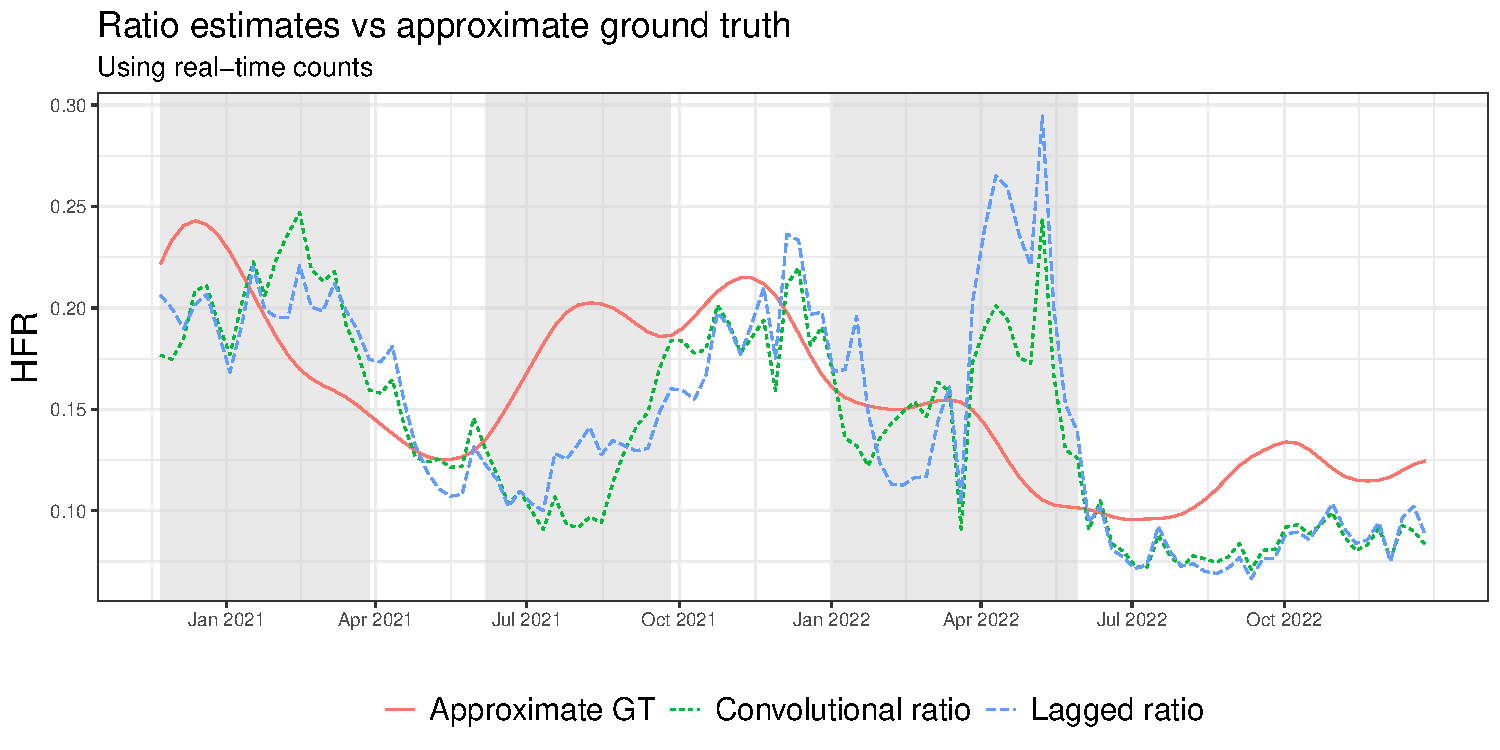
\includegraphics[width=\linewidth]{Figures/Real/US_ests_realtime.pdf}
  \caption{Convolutional and lagged ratios against approximate ground truth
    HFR.} 
\end{subfigure}

\bigskip
\begin{subfigure}[b]{\linewidth}
  \centering
  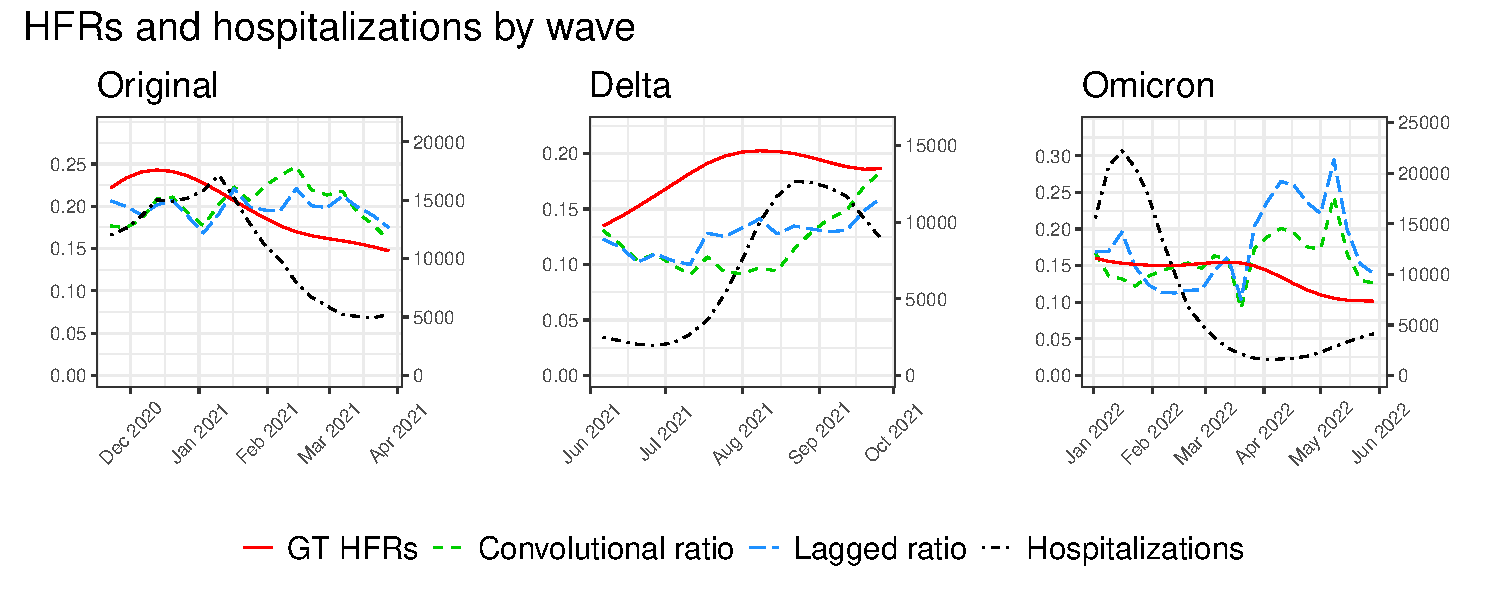
\includegraphics[width=\linewidth]{Figures/Real/hfrs_by_wave.pdf}
  \caption{Zooming in to focus on major variants, with hospitalizations overlaid
    (right y-axis).}
\end{subfigure}

\caption{Comparing ratio estimates to approximate ground truth HFR on real
  COVID-19 data in the US, from November 2020 through December 2022.}
\label{fig:basic_est_vs_gt_figs}
\end{figure}

Overall, both ratio estimators perform poorly. Their bias is consistent and
nontrivial, especially for the lagged estimator. Both respond very slowly to
changes in the HFR. As the HFR declines following the wave in winter 2021, both   
ratios hover near 20\% for several months. More troublingly, they are too slow
to detect the rise in HFR in the early Delta period (summer 2021). If the
purpose of these estimators is to inform stakeholders of increased risks in real
time, they failed during the Delta surge.  

The most significant bias comes in the middle of the Omicron wave in spring
2022. In this period, the HFR remains around 15\% until April, then sharply
declines to 9\% two months later. The ratio estimates first fluctuate around the
true HFR, and then subsequently, both estimates surge as the true HFR nears
its nadir, with the lagged ratio approaching 30\%. This dramatic upswing signals
a serious false alarm.  The analysis in Sections \ref{sec:wellspecified} and
\ref{sec:misspecified} explain each of these failure cases. 

\paragraph{Well-specified analysis.}

We start by analyzing the convolutional ratio with respect to the well-specified
bias expression in Proposition \ref{prop:OracleBias}. While this expression
assumes that the true delay distribution is known, we found that different
choices of delay distribution generally yield similar bias (Appendix
\ref{apx:robustness}). This indicates that our convolutional ratio may 
not be far from the oracle (well-specified) ratio. 

Proposition \ref{prop:OracleBias} indicates that the bias moves in the opposite
direction of the true severity rate. This occurs during the Delta wave, when the
HFR rises well before the ratio estimates do. On the other hand, falling HFR
produces positive bias, as observed in the original and Omicron waves.  

The enormity of the bias during Omicron can partially be attributed to the
precipitous decline in hospitalizations, as falling primary incidence has been
shown to exacerbate the bias. Average daily hospitalizations declined from over
20,000 in mid-January to only 1,500 by April 1. Lastly, the delay distribution
is relatively heavy-tailed, because the aggregate deaths here (from JHU) are
aligned by report date. We find that this has a substantial impact on the bias, 
as analyzed in Appendix \ref{apx:alternatives}.

\paragraph{Misspecified analysis.}

The misspecification analysis explains central discrepancies between the
convolutional and lagged ratios. Section \ref{sec:misspecified} discusses why we 
expect \smash{$A_t^\ell < 1$} around the start of a decline in primary
incidence. As a result, the lagged ratio will incur negative misspecification
bias, and we observe this when hospitalizations with the original variant
decline from their peak in mid-January 2021. Throughout February, lagged
estimates are about 2\% below the positively biased convolutional ratios.   

As primary incidence rises, we expect \smash{$A_t^\ell > 1$}, contributing
positive bias relative to the (approximately) well-specified convolutional
ratio. Correspondingly, when hospitalizations surge due to the Delta variant in 
August 2021, the lagged ratio is less negatively biased. Lastly, recall, we
expect \smash{$A_t^\ell > 1$} \emph{after} a fall in primary incidence. This
accounts for the lagged ratio having higher bias in April 2022, when
hospitalizations level out from the Omicron surge. There, the lagged HFR (and 
presumably also the misspecification factor \smash{$A_t^\ell$}) hits its maximum
value.   

\paragraph{}

We performed several robustness checks to assess the stability of these
findings. Appendix \ref{apx:robustness} studies the effect of different
hyperparameter choices, and also examines the ratio estimators on six US
states. It also compares HFR estimates using finalized counts, rather than the
data available in real time. By and large, the ratio estimators yield roughly
the same type of bias throughout.

\subsection{Simulated data}\label{sec:results_sim}

We further evaluated these methods in a variety of simulation settings. Given a series of time-varying HFRs $p_t$ and delay distribution $\pi$, deaths are defined without noise from \eqref{eq:model}:
$$Y_t = \sum_{k=0}^d X_{t-k} \P(\text{die at $t$}\given\text{hosp at }t-k) = \sum_{k=0}^d X_{t-k} \pi_k p_{t-k}.$$

Like the experiments in Sections~\ref{sec:wellspecified} and~\ref{sec:misspecified}, we
used real-time HHS hospitalization counts. The simulations in this
section evaluate performance over a two-year period, with a broader range of
underlying HFR curves. To supplement the NHCS HFRs, we mimicked the opposite
trend by inverting and rescaling them. We also modeled a stationary HFR of 10\%
over all time. As in Section~\ref{sec:setup}, the delay distributions were again
gamma with standard deviation 0.9 of their mean. We experimented with means of
12 and 24 to illustrate a short and long delay distribution. 

To elucidate the oracle bias in Proposition \ref{prop:OracleBias}, we let the convolutional ratio use the true delay distribution. For the lagged ratio, $\ell$ was again chosen to maximize the cross-correlation between hospitalizations and deaths. We also experimented with the mean of the delay distribution, as advocated by \citet{lagged_chinese}. Figure \ref{fig:sims_mean_lag} in Appendix~\ref{apx:misc} shows the results are similarly unstable.


\begin{figure}
    \centering
    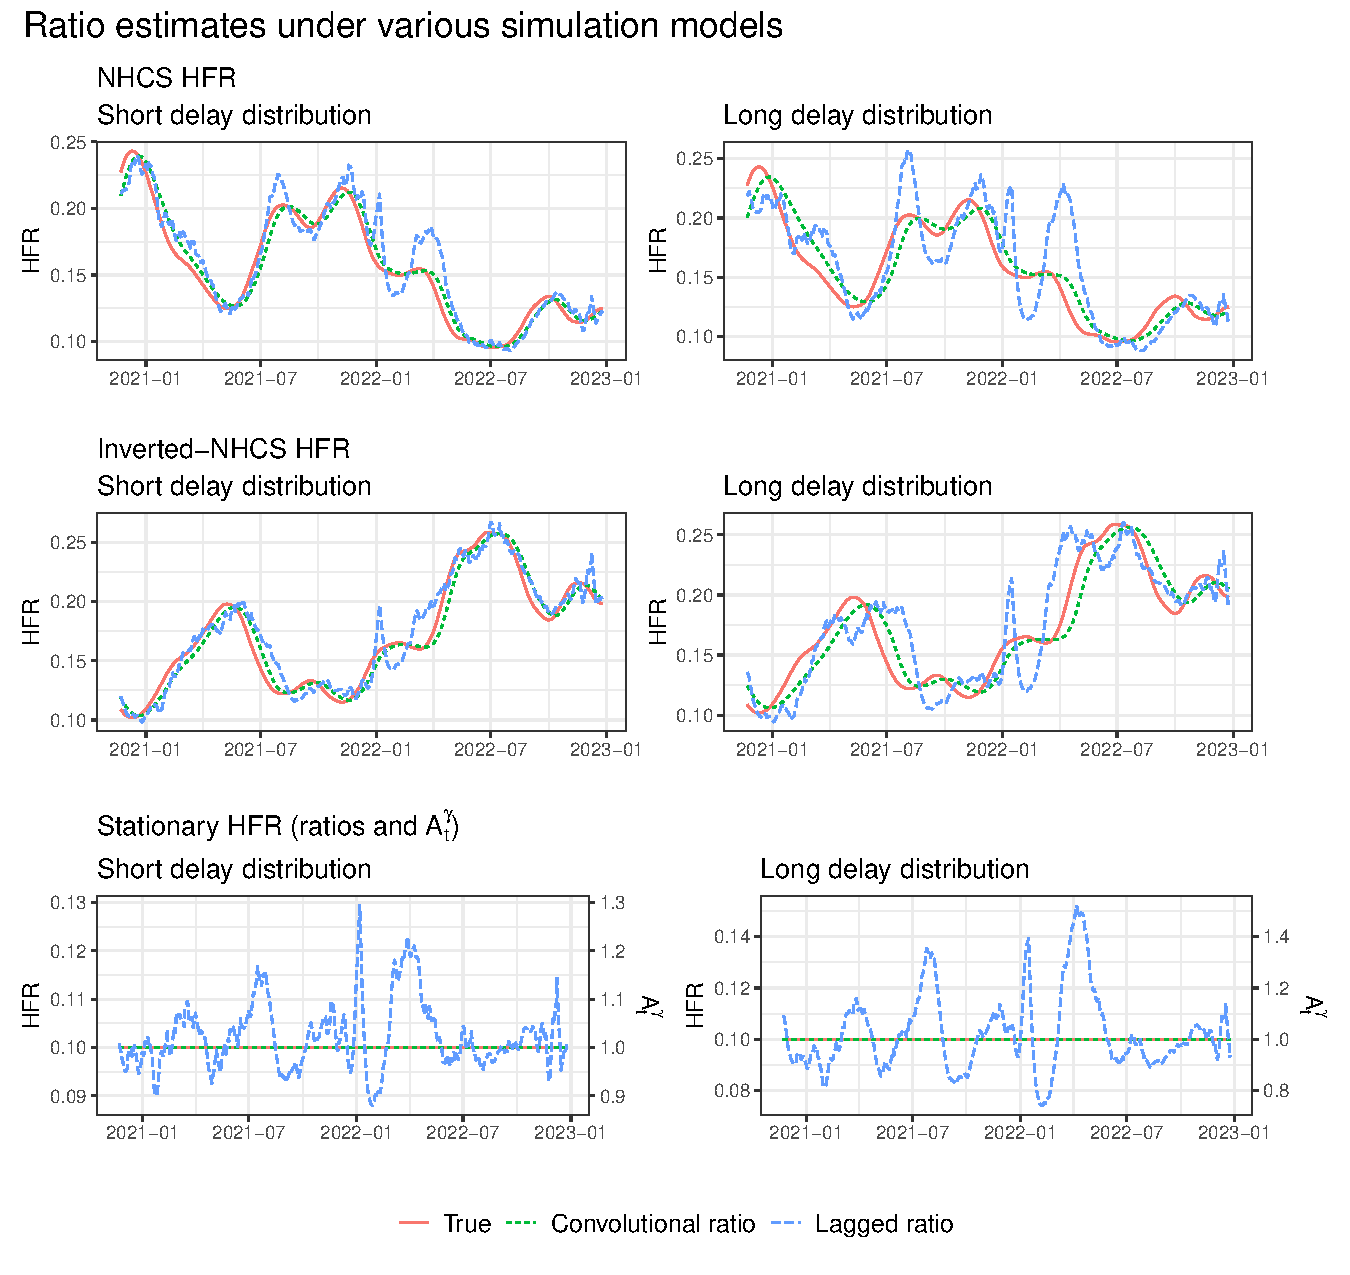
\includegraphics[width=\linewidth]{Figures/Simulated/simulated_results_corr_lag.pdf}
    \caption{True and Estimated HFRs from Simulated Deaths. First column has short delay distribution, second has long.}
    \label{fig:sims}
\end{figure}

Figure \ref{fig:sims} displays the results on the six settings of delay distribution and HFR. 
% Consequently, $\hat{p}_t^\gamma = p A_t^\gamma$. 
%so the $A_t^\gamma$ curve merely rescales the estimated HFRs by a factor of $p$. 
Matching expectations, HFRs are significantly more biased given the longer underlying delay distribution. 
In all three HFR settings, the lagged ratios swing more widely. For example, when the true HFR is a constant 10\%, they peak at 12\% under the light-tailed distribution, compared to 15\% with the heavy tail. The oracle convolutional ratio does not share the lagged estimator's dramatic oscillations. Rather, it tracks the general shape of true curve, albeit at a delay. For the NHCS HFRs, the average delay was 5 days for the light-tailed distribution, and 12 days with heavy tail; these delays were 6 and 14 days for the inverted curve. (To compute the average delay, we again took the maximal cross-correlation between the two series.)

% In general, the oracle convolutional ratio performs much better than the lagged estimator. Our analysis accounts for this wide gap in performance. In the case of a stationary severity rate, for example, Proposition \ref{prop:OracleBias} assures the oracle convolutional ratio is unbiased. But if the delay distribution is misspecified, Proposition \ref{prop:MispBias} expresses the resulting bias via the ratio $A_t^\gamma$. This quantity does not depend on the severity rate, so the bias moves in similar trajectories across the three HFR settings. 
% In general, the oracle convolutional ratio is much more accurate than the lagged estimator. 
The analysis in Section~\ref{sec:misspecified} accounts for the wide gap in performance between the two estimators. 
%The lagged bias moves in ways that align with our observations. 
% Proposition \ref{prop:MispBias} expresses bias under misspecification via the rescaled oracle bias plus a misspecification term, both of which depend on the ratio $A_t^\gamma$. 
Proposition \ref{prop:MispBias} expresses bias under misspecification as a function of the factor $A_t^\gamma$. 
These ratios $A_t^\gamma$ are visualized in Figure \ref{fig:sims} as rescaled HFR estimates in the stationary case.
% In addition to the HFR curves, it also visualizes the ratios $A_t^\gamma$, which merely rescale the HFR estimates in the stationary case. 
Given a constant rate $p$, the oracle convolutional ratio is unbiased, so Proposition \ref{prop:MispBias} reduces to $\mathbb{E}[\hat{p}_t^\gamma] = p A_t^\gamma$. Furthermore, $\mathbb{E}[\hat{p}_t^\gamma] = \hat{p}_t^\gamma$, as our setup simulates deaths without noise. Consequently, $A_t^\gamma = \frac{\hat{p}_t^\gamma }{p}$. 

In expectation, the lagged ratio is higher than the oracle convolutional ratio when $A_t^\gamma>1$, and lower when $A_t^\gamma<1$. Comparing the $A_t^\gamma$ curves to the estimated HFRs, the bias moves very similarly. 
For example, 
% The analysis in Section~\ref{sec:misspecified} explains these trajectories. During
during the Delta and Omicron waves, rapid rises in hospitalizations produced high values of $A_t^\ell$. This accounts for the spikes in August 2021 and January 2022. %, across all 3 HFR settings
When hospitalizations level out from the Omicron surge, $A_t^\ell$ spikes to 1.2 and 1.5 for the short and long distributions --- hence the positive bias in spring 2022. 
% Positive bias is also expected when hospitalizations have leveled out from a decline. This consistently occurs in spring 2022, with $A_t^\ell$ reaching 1.2 and 1.5 for the short and long distributions. 
Lastly, the lagged estimator should have negative bias as primary events fall. We observe this in Delta (September 2021) and Omicron (Februrary 2022). 

% Not sure if these two paragraphs belong in the discussion. They're analytical, but don't belong in Section 2.4 because they rely on these empirical results. 
The misspecified bias (Proposition \ref{prop:MispBias}) rescales the oracle bias and adds a misspecification term. Studying Figure \ref{fig:sims}, we observe the misspecification term tends to dominate when $A_t^\gamma$ strays away from 1. To understand this, consider periods in which the oracle bias is negative. As introduced in Section~\ref{sec:misspecified}, the oracle and misspecification terms are at odds with each other when this is the case. 
% When $A_t^\gamma > 1$, it both amplifies the negative oracle bias and adds positive misspecification bias. The opposite effect occurs when $A_t^\gamma<1$. 
% $A_t^\gamma > 1$ amplifies the negative bias while adding positive misspecification bias, whereas $A_t^\gamma<1$ has the opposite effect.

Invariably, the lagged ratio moves in the direction of the misspecification term $p_t(A_t^\gamma-1)$. Under the true NHCS HFRs, for example, the lagged estimates spike with $A_t^\ell$ in August 2021. In the inverted setting, the lagged bias tracks the down-up-down motion of $A_t^\ell$ during the first five months of 2021. That the misspecification term wins out in these conflicting settings indicates it comprises a disproportionate amount of the bias. Indeed, the oracle bias is generally low enough that multiplicative rescaling may not have a large effect.

For a further example, consider the bias at April 2022 on the middle right. The true HFR is 14\%, with the convolutional ratio nearby at 15\%. Meanwhile, the lagged ratio peaks at 22.5\%, driven upwards by an $A_t^\ell$ of $1.5$. Decomposing the lagged bias of $8.5\%$ with Proposition \ref{prop:MispBias}, the oracle term $A_t^\ell \text{Bias}(\hat{p}_t^\pi)$ equals only $1.5\%$; meanwhile, the misspecification term $p_t(A_t^\ell-1) = 7\%$, accounting for the majority of the bias. 

\section{Discussion}

Our analyses illustrate that practitioners should take caution when using
time-varying severity ratio estimators. They exhibit considerable bias when severity rates
change, particularly the popular lagged ratio estimator. A major purpose of these
estimators is to inform stakeholders of changing risks in real time; this bias
indicates they may fail to do so in a reliable manner.

% It may not be possible to infer about the oracle bias, since the true severity rates are unknown. However, understanding the central importance of the misspecification term in Proposition \ref{prop:MispBias} enables us to make broad heuristics about biases observed in practice. 
Analyzing the lagged ratio enables us to make real-time heuristics about its performance in practice. Proposition \ref{prop:MispBias} decomposes its bias into oracle and misspecification terms, the latter of which has been shown to dominate. Based solely on the primary incidence curve, we can expect the lagged ratio to make the following errors:
\begin{enumerate}
    \item Unreasonably high severity estimates when primary incidence is rising quickly;
    \item Rapid declines when primary incidence is falling quickly;
    \item Unexpected surges when primary incidence has leveled out after falling. 
\end{enumerate}

Practitioners can adjust their reactions accordingly when these bias patterns occur in real time. For example, if the lagged HFR spikes shortly after hospitalizations reach a stable low, a savvy epidemiologist can temper her alarm with the knowledge it may well be spurious.

While the lagged ratio is ubiquitous in practice, our analysis of its
drawbacks suggests other aggregate estimators should be favored. Figure
\ref{fig:sims} showed the oracle convolutional ratio is much more
accurate. 
% Even with a rough estimate of the delay distribution, 
% it generally displayed improved stability and performance (Figures \ref{fig:misspecified},
% \ref{fig:basic_est_vs_gt_figs}, and \ref{fig:sims}) --- though it still has large bias.
It still outperformed the lagged ratio given a misspecified delay distribution, though its bias was also large (Figures \ref{fig:misspecified} and \ref{fig:basic_est_vs_gt_figs}).
% While \eqref{eq:nish} from \citet{nishiura} is widely used to compute stationary or
% average HFRs, we have not come across any applications for the time-varying
% case.


% Given the drawbacks of these methods, alternative approaches may be preferable when there is reason to believe the true rate is changing. If possible, severity rates can be obtained from line-list data after accounting for right censoring. These rates can then be scaled to a broader population with careful demographic adjustment \citep{verity2020estimates}. 

% More commonly, only aggregate data is available, especially in real time. In that case, other methods may outperform these ratios. \citet{fusedlasso} propose estimating all severity rates at once with a Fused Lasso model, using the relation in \eqref{eq:model}. Unlike the other approaches, this method is inherently forward-looking, where rates at $t$ are exclusively used to produce secondary events after $t$. However, it may suffer from other sources of bias. It is inclined to estimate smoothly-changing severity rates as piecewise constant, and may yield unstable real-time estimates due to scarce data at the tail.

% \citet{fusedlasso} proposed a alternative approach which differs sharply from the ratios discussed in this paper. 
\citet{fusedlasso} proposed an approach that differs considerably from the ratios discussed in this paper. 
The method estimates all historical severity rates at once, using the relation in \eqref{eq:model} to fit a fused lasso model. This estimator is inherently forward-looking, where rates at $t$ are exclusively used to produce secondary events after $t$. Given regularization parameter $\lambda$, current time $T$, and start time $t_0$, the fused lasso estimates

$$\hat{p}^\text{FL} = \text{argmin}_{p \geq 0} \sum_{t=t_0}^T (Y_t-\sum_{j=0}^d X_{t-j}\gamma_j p_{t-j})^2 + \lambda\sum_{t=t_0-d+1}^{T}\lvert p_t - p_{t-1}\rvert.$$

This estimator is not succumb to the issues of the backward-looking ratios. However, it may suffer from other sources of bias. It is inclined to estimate smoothly-changing severity rates as piecewise constant, and may yield unstable real-time estimates due to scarce data at the tail. 
Thorough investigation of its performance is a promising object for future study.

Future work could generalize the above approach beyond piecewise constants. The fused lasso is a special case of trend filtering, a nonparametric regression technique that fits piecewise polynomials \citet{Tibshirani2014}. Higher-order curves may better model trends and improve performance. \citep{Jahja2022} applies trend filtering to a similar deconvolution problem, reconstructing latent infections from case reports. Its insights on tail regularization may be useful to stabilize severity estimates. 

\citet{UKpaper} also proposed a forward-looking method, this one a ratio between relevant primary and secondary events. However, this method is not applicable in real time, as it uses secondary events after $t$ to compute the severity rate. Nevertheless, it is a useful tool for retrospective estimation. 

Another retrospective tool is aggregate COVID deaths from NCHS, a resource that
was not available in real time (Appendix~\ref{apx:NCHS_deaths}). Unlike JHU,
whose aggregates align deaths by report date, NCHS counts deaths on the day the
actually occurred. As a result, the mean of its delay distribution is
considerably lower, so it produces more accurate ratio estimates (Figures
\ref{fig:sims} and \ref{fig:jhu_vs_nchs}). Analogously, bias is a more serious
issue with earlier primary events. For example, case- or infection-fatality
ratios may be more biased than hospitalization-fatality ratios. 

Severity rates may be biased in ways beyond the statistical bias our work
focuses on. 
In Section~\ref{sec:setup}, we mentioned that 
HFR estimation from aggregates is subject to survivorship bias --- 
the failure to account for deaths that occurred outside the hospital \citep{lipsitch2015potential}.
% Section~\ref{sec:setup} mentioned, for example, the fact that
% estimating HFR from aggregates fails to address the large proportion of deaths
% that occur outside the hospital; \citep{lipsitch2015potential} refers to this as
% ``survivorship bias." 
Under-reporting is another central challenge, particularly for CFR.
% Another central challenge, this one for CFR estimation, is under-reporting.
Not all infections are reported, reporting rates change across time, and severe
cases are more likely to be reported than mild cases.
\citet{reich2012estimating} proposed an estimator for a time-invariant
\emph{relative} CFR --- the ratio of CFRs between groups --- that learns these
latent reporting rates via the EM algorithm \citep{EM}. \citet{anastasios}
applied this in the context of COVID-19, analyzing how the chosen delay
distribution affects its results. The work also identifies other sources of bias, like
differences in case definition and testing eligibility.


% As defined in \eqref{eq:severity}, the severity rate is analogous to case $R_t$. Both concern the average number of secondary events produced by a primary event at time $t$. Moreover, the real-time severity ratios we study are analogous to instantaneous $R_t$, both of which measure how primary events in the past contribute to secondary events at $t$. Indeed, one of the most popular frameworks for estimating instantaneous $R_t$ is strikingly similar to the convolutional ratio \citep{fraser2007,wallinga2007how,cori2013new,rtestim}:
% \begin{equation}\label{eq:instRt}
%     \hat{R_t} = \frac{I_t}{\sum_{k=0}^d I_{t-k}g_k}.
% \end{equation}
% The most fundamental difference between Eq. \eqref{eq:instRt} and \eqref{eq:conv} is the former expresses the rate for a single time series. 
As discussed in Section~\ref{sec:defs}, severity rates may be understood in connection with reproduction numbers. This connection extends to their bias as well. For example, we  demonstrated that the convolutional ratio is unbiased if the severity rate and delay distribution in the $d$ days before $t$ are stationary. In a similar vein, \citet{fraser2007} noted that instantaneous $R_t$ is equal to case $R_t$ if conditions remain unchanged. 
Future work along the lines of \citet{rt_study} could apply our analytical framework to $R_t$ bias, examining the fidelity of instantaneous $R_t$ as a proxy for case $R_t$. 

\bibliographystyle{apalike}
\bibliography{refs}

\clearpage
\appendix

\section{Proofs and further analysis}
\label{apx:proofs}

\subsection{Proof of Proposition \ref{prop:OracleBias}}
\label{apx:OracleBias}

Here and henceforth, we abbreviate \smash{$\E_t[\cdot] = \E[\cdot \given
  \{X_s\}_{s\leq t}]$}. Observe that
\begin{align*}
\bias(\hat{p}_t^\pi) 
&= \frac{\E_t[Y_t]}{\sum_{k=0}^d X_{t-k}\pi_k} - p_t \\ 
&= \frac{\sum_{k=0}^d X_{t-k}\pi_k p_{t-k}}{\sum_{k=0}^d X_{t-k}\pi_k} - 
\frac{p_t \sum_{k=0}^d X_{t-k}\pi_k}{\sum_{k=0}^d X_{t-k}\pi_k} \\
&= \sum_{k=0}^d \frac{X_{t-k}\pi_k}{\sum_{j=0}^d X_{t-j}\pi_j} (p_{t-k}-p_t).
\end{align*}

% The well-specified bias can be understood as a weighted average of
% $\{p_{t-k}-p_t\}_{k=0}^d$. The attainable absolute bias ranges between
% $\min_{k=0, \dotsc, d} |p_{t-k}-p_t| = 0$, achieved by $k=0$, and $\max_{k=0, 
%   \dotsc, d} |p_{t-k}-p_t|$. This maximal bias is achieved by setting one of
%   the weights $X_{t-k}\pi_k/(\sum_{j=0}^d X_{t-j}\pi_j)$ to 1 and the rest to
%   zero, either through the delay distribution $\pi$ or through the primary
%   incidence curve $X$. Hence, the explanations for delay distribution and
%   primary incidence are aligned: They inflate the bias by upweighting distant
%   timepoints for which the severity rate was different. If severity rates are
%   monotonically changing, for example, th en the maximal bias occurs at $k=d$.  

\subsection{Proof of Proposition \ref{prop:MispBias}}
\label{apx:MispBias}

Observe that
\begin{align*}
\bias(\hat{p}_t^\gamma) 
&= \frac{\E_t[Y_t]}{\sum_{k=0}^d X_{t-k}\gamma_k} - p_t \\
&= \frac{\sum_{k=0}^d X_{t-k}\pi_k p_{t-k}}{\sum_{k=0}^d X_{t-k}\gamma_k} -
\frac{\sum_{k=0}^d X_{t-k}\gamma_k p_t}{\sum_{k=0}^d X_{t-k}\gamma_k} \\
&= \sum_{k=0}^d \frac{X_{t-k}}{\sum_{j=0}^d X_{t-j}\gamma_j}
(\pi_k p_{t-k} - \gamma_k p_t) \\
&= \sum_{k=0}^d \frac{X_{t-k}}{\sum_{j=0}^d X_{t-j}\gamma_j}
(\pi_k p_{t-k}-(\pi_k +(\gamma_k-\pi_k)) p_t) \\
&= \frac{\sum_{j=0}^d X_{t-j}\pi_j}{\sum_{j=0}^d X_{t-j}\gamma_j}
\sum_{k=0}^d \frac{X_{t-k}\pi_k}{\sum_{j=0}^d X_{t-j}\pi_j}(p_{t-k}-p_t) -
p_t\sum_{k=0}^d \frac{X_{t-k}}{\sum_{j=0}^d X_{t-j}\gamma_j}(\gamma_k -\pi_k) \\ 
&= \frac{\sum_{j=0}^d X_{t-j}\pi_j}{\sum_{j=0}^d X_{t-j}\gamma_j} 
\bias(\hat{p}_t^\pi) + p_t\Bigg( \frac{\sum_{k=0}^d X_{t-k}\pi_k} 
{\sum_{j=0}^d X_{t-j}\gamma_j}-1\Bigg).
\end{align*}

\subsection{Further analysis of \eqref{eq:OracleBias}}
\label{apx:analysis}

We present examples that further explain the well-specified bias. These are more
contrived that the ones in Section \ref{sec:wellspecified}, for example, using
unrealistic delay distributions. Nonetheless, their bias can be simplified to 
simple analytic formulas, isolating the three contributing factors. 

To elucidate the relationship between changing severity rates and bias, let us
consider the case where all secondary events occur after precisely $\ell$ time  
points. Note, the well-specified convolutional and lagged ratio estimators
coincide: \smash{$\hat{p}_t^\gamma = \hat{p}_t^\ell = p_{t-\ell}$}. The bias in
this setting is simply the change in the true severity rate, $p_{t-\ell} - p_t$, 
and the ratio estimator is unbiased only if the severity rate is stationary. 
Otherwise, say, the ratio will be 20\% too low if the true severity rate was
20\% lower $\ell$ time steps ago. 

Typically, severity rates will be less similar to the present value $p_t$ as we
go further back in time, thus, for  example, the bias $p_{t-\ell}-p_t$ will be
generally larger when $\ell=28$ versus $\ell=14$. This supports the general idea
that estimates with heavier-tailed delay distributions tend to have more bias.          

Now to elucidate the relationship between primary incidence and bias, let us 
consider a delay distribution $\pi$ which places half its mass at lag 0, and the
other half at lag $q$. Then the bias \eqref{eq:OracleBias} has magnitude:
\[
\big| \bias(\hat{p}_t^{\gamma}) \big| = \frac{\frac{1}{2} \big| X_t(p_t-p_t) +
  X_{t-q}(p_{t-q}-p_t) \big|} {\frac{1}{2}(X_t+X_{t-q})} = \frac{|p_{t-q}-p_t|}
{1 + X_t / X_{t-q}}. 
\]
In other words, the absolute bias is monotonically decreasing in
$X_t / X_{t-q}$, the proportion change in primary incidence. Rising  
primary incidence ($X_t / X_{t-q} > 1)$ yields less bias, while falling 
levels yield more. 

% Figure \ref{fig:chging_primary} displays this setting. Hospitalizations are
% defined as $X = \sigma(s)*9000+1000$, where $\sigma$ is the sigmoid function
% and $s$ takes 300 evenly spaced steps from -9 to 7. The true HFRs fall from
% 0.5 to 0 over the same number of even steps. Indeed, the convolutional ratio's
% bias dips as hospitalizations rise, and rises as they fall.  

% The figure also plots with lagged ratio with $\ell=\frac{d}{2}$, the mean of
% the delay distribution. When daily hospitalizations are close to constant, the
% two estimators converge towards the same ratio. During periods of change,
% however, the lagged estimator has different bias. It first moves upwards ---
% the opposite direction as the convolutional bias --- with far greater
% magnitude. This can be explained by the ratio $A_t^\ell =
% \frac{X_{t-2\ell}+X_t}{2X_{t-\ell}}$ from Proposition \ref{prop:MispBias}. As
% hospitalizations begin to steeply rise, $X_{t-2\ell}$ and $X_{t-\ell}$ are
% similar, but $X_t > X_{t-\ell}$. Hence, $A_t^\ell>1$, contributing positive
% bias to both the oracle and misspecification terms. As hospitalizations level
% out near the top, $A_t^\ell < 1$, hence the bias falling lower. The opposite
% pattern occurs as hospitalizations fall.  

% \begin{figure}[tb]
% \centering
% \begin{subfigure}[b]{0.495\linewidth}
%   \centering
%          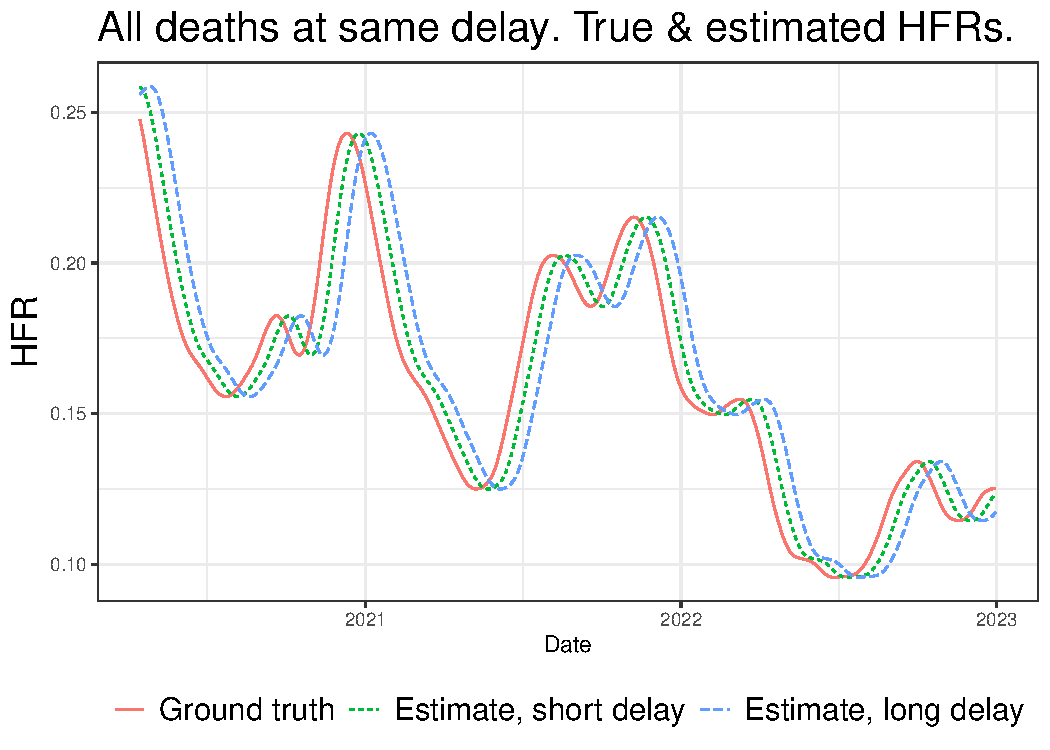
\includegraphics[width=\linewidth]{Figures/Simulated/sim_onehot.pdf} 
%          \caption{All deaths after $\ell$ days. HFR ratios equivalent;
%          plotting delays of $\ell=14$ and 28 days.} 
%          \label{fig:onehot}
%      \end{subfigure}
%      \hfill
%      \begin{subfigure}[b]{0.495\linewidth}
%          \centering
%          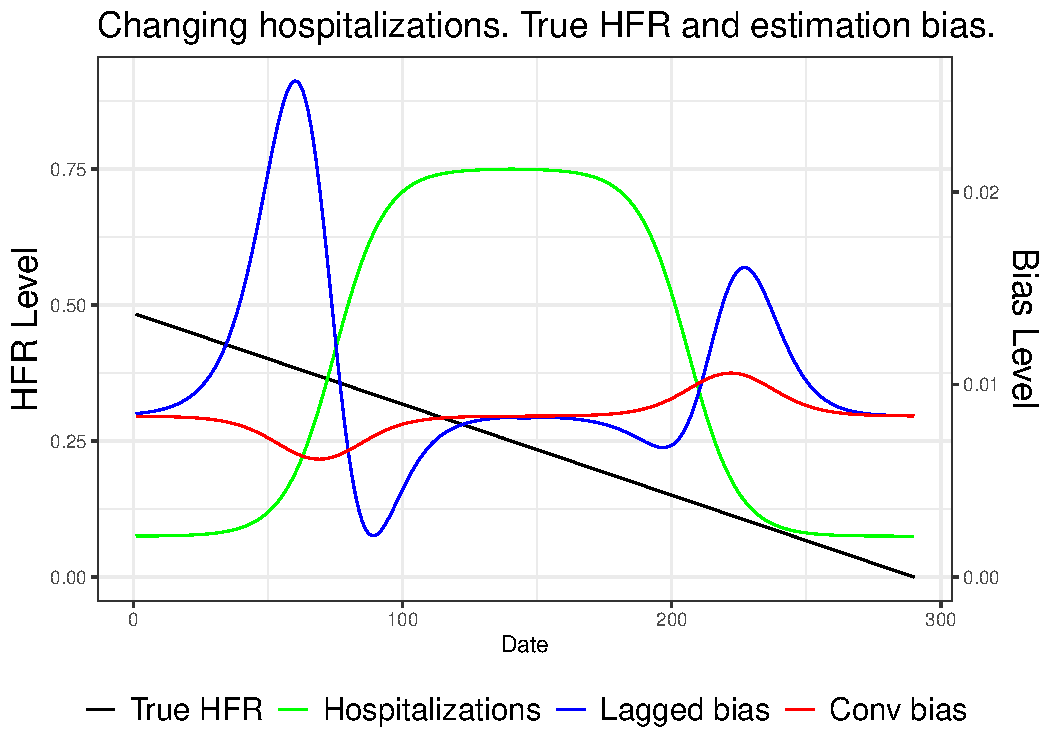
\includegraphics[width=\linewidth]{Figures/Simulated/sim_chging_primary.pdf} 
%          \caption{Changing primary incidence. Plotting bias of lagged and
%          convolutional ratios.} 
%          \label{fig:chging_primary}
%      \end{subfigure}
%         \caption{Toy examples of biased severity rates.} 
%         \label{fig:bias_ex}
% \end{figure}

% Since the convolutional ratio uses the true delay distribution, it has oracle
% bias in Proposition \ref{prop:MispBias}. The lagged ratio has lag at the mean
% of the delay distribution, $\ell=\frac{d}{2}$. Its behavior can be explained
% by the ratio $A_t^\ell = \frac{X_{t-2\ell}+X_t}{2X_{t-\ell}}$. As
% hospitalizations begin to steeply rise, $X_{t-2\ell}$ and $X_{t-\ell}$ are
% similar, but $X_t > X_{t-\ell}$. Therefore $A_t^\ell>1$, inflating the
% positive oracle bias term and adding misspecification bias. As
% hospitalizations level out near the top, $A_t^\ell < 1$, hence the bias
% falling lower. The opposite pattern occurs as hospitalizations fall. 

\section{Alternative data sources}
\label{apx:alternatives}

\subsection{Retrospective deaths}
\label{apx:NCHS_deaths}

JHU aggregated daily deaths in real time, aligned by the date they were
reported. In contrast, the National Center for Health Statistics (NCHS) provided
weekly totals of deaths aligned by occurrence, which were not available in real  
time. Intuitively, the delay which relates hospitalization to death occurrence
should have a lighter tail in comparison to that relating hospitalization to
death report. Therefore, since that heavier-tailed delays generally introduce
greater bias, we would expect ratio estimates computed from JHU deaths to have
greater bias than those from NCHS deaths. Figure \ref{fig:jhu_vs_nchs} shows
that this is indeed the case. Using NCHS data---which was only available in
retrospect---leads to lagged HFR estimates with significantly less bias.  

\begin{figure}[h]
\centering
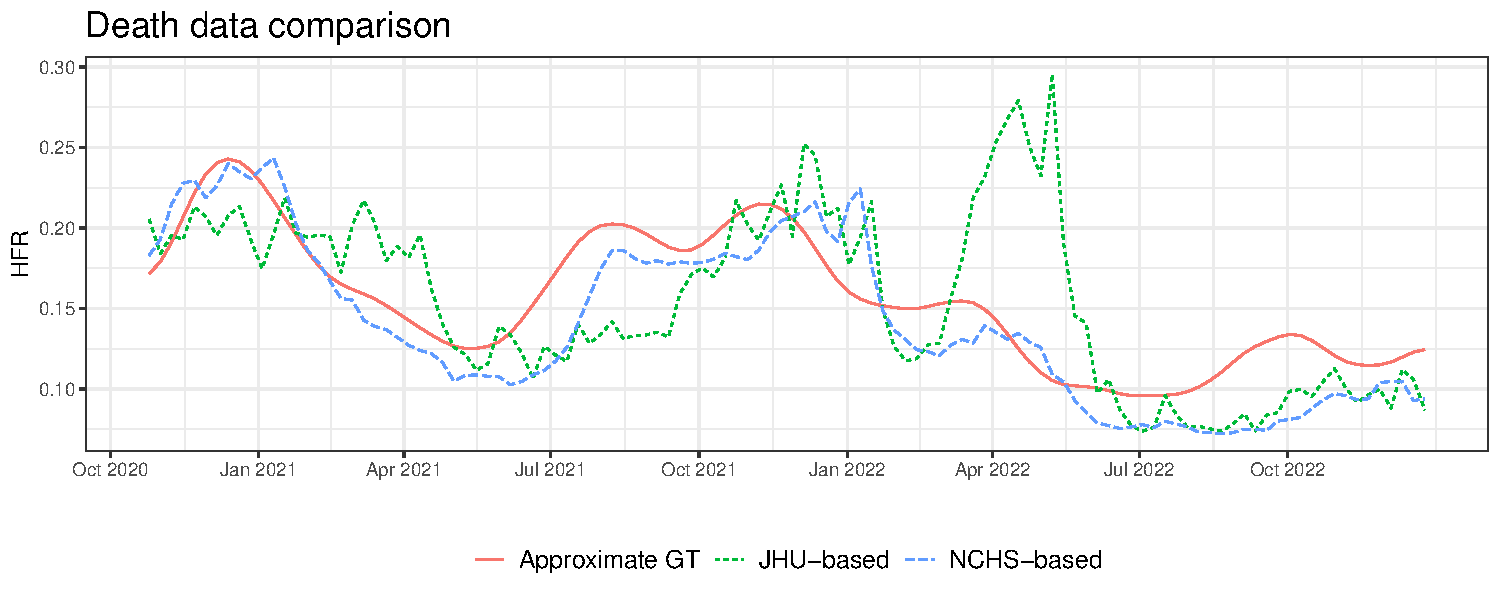
\includegraphics[width=\linewidth]{Figures/Real/jhu_vs_nchs.pdf}
\caption{Comparing lagged ratios based on data from JHU versus NCHS.}
\label{fig:jhu_vs_nchs}
\end{figure}

\subsection{Alternative ground truth}
\label{apx:alt_gt}

\begin{figure}[b!]
\centering
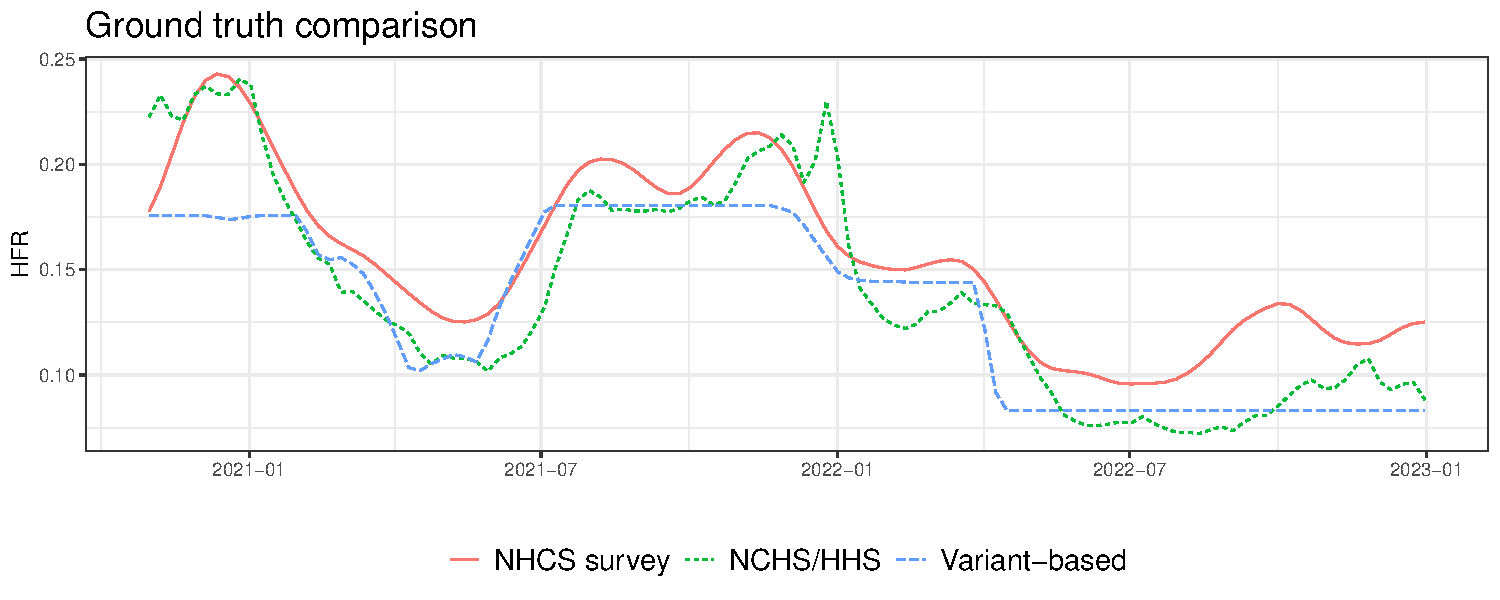
\includegraphics[width=\linewidth]{Figures/Real/ApproxGT.pdf}
\caption{Comparing methods for approximating ground truth HFR.}
\label{fig:approxGT}
\end{figure}

We consider two alternative approaches to approximate the ground truth HFR
curve, over the COVID-19 pandemic. The first is simply to use the lagged ratio
based on NCHS data. As discussed above, this benefits from a lighter-tailed
delay distribution than JHU data. Further, as we are looking to approximate
ground truth in retrospect, we modify this estimator to be forward-looking:
\smash{$\hat{p}_t^\ell = Y_{t+\ell} / X_t$}. The second approach we consider is
to compute a single HFR by dividing total deaths by total hospitalizations in
each major variant period,  
% during the period where it accounted for over 50\% of activate cases 
and then create a smooth curve by mixing these per-variant HFRs by estimates of 
the proportion of variants in circulation, obtained from CoVariants.org
\citep{Hodcroft2021}. We only considered the four largest variants: the original
strain, Alpha, Delta, and Omicron. However, because Omicron began with an
enormous surge that quickly subsided, we split it into early and late periods,
following \citep{adjei2022mortality}.     

Figure \ref{fig:approxGT} displays these two alternative ground truth curves,
alongside that obtained from NHCS. They have nontrivial differences in
magnitude, but reassuringly, move more or less in conjunction. The retrospective
NCHS ratios will still be subject to statistical bias (similar to
\eqref{eq:LagBias}). The variant-based HFRs are flatter, as they do not account
for other sources of (potential) variability in the underlying severity rate.


\section{Robustness checks}
\label{apx:robustness}

\subsection{Real-time versus finalized data}

Recall, the results in Section \ref{sec:results_real} use hospitalization and
death counts available in real time. To investigate the sensitivity of our
findings, we recomputed the lagged and convolutional ratios, this time using
finalized counts. Figure \ref{fig:rt_and_final} shows the real-time and
finalized estimates track one another very closely. Therefore, the observed bias
in Figure \ref{fig:basic_est_vs_gt_figs} cannot be attributed to real-time
reporting quirks.  

% The one period where the curves are significantly different from one another
% is in March 2022. While the HFRs from finalized counts steadily rise, the
% real-time estimates sharply fall then immediately bounce back. This sudden
% drop is due to a brief period in which reported death counts were suddenly too
% low (Fig. \ref{fig:source}. This is corrected in the finalized counts, hence
% their smooth HFRs. Removing this artifact further reinforces the bias trends
% described in Section~\ref{sec:wellspecified}. 

\begin{figure}[htb]
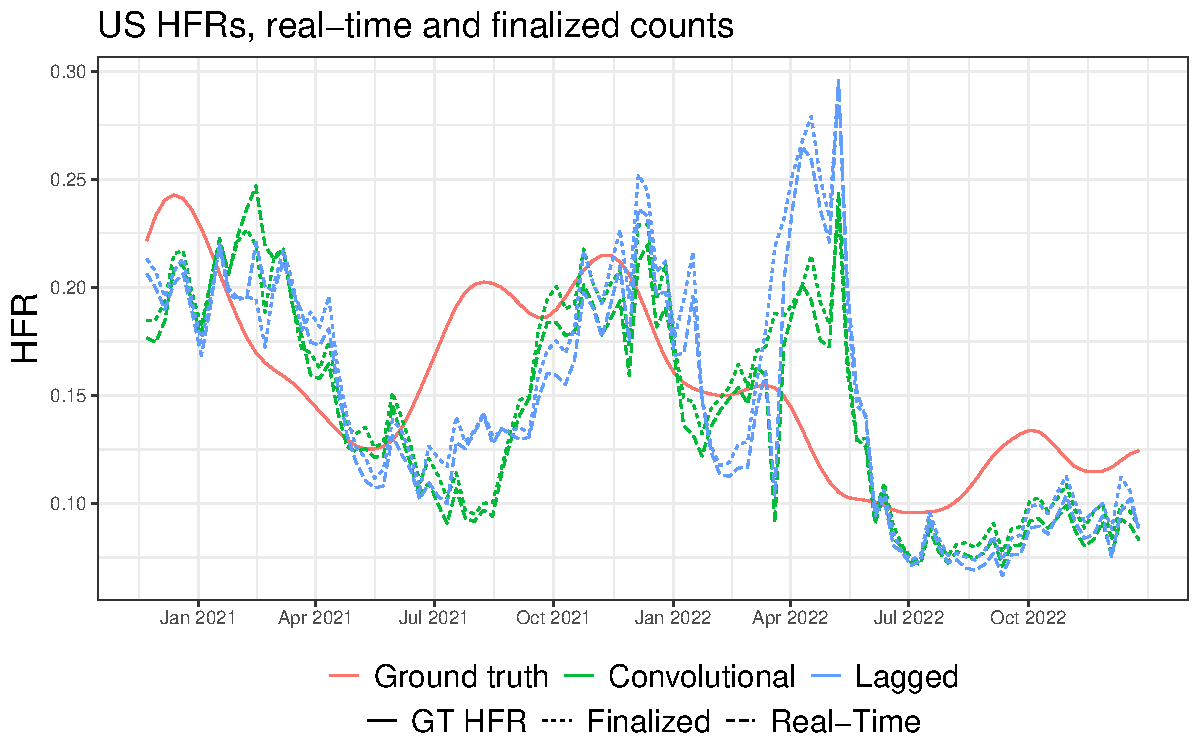
\includegraphics[width=\linewidth]{Figures/Real/US_ests_realtime_both.pdf}
%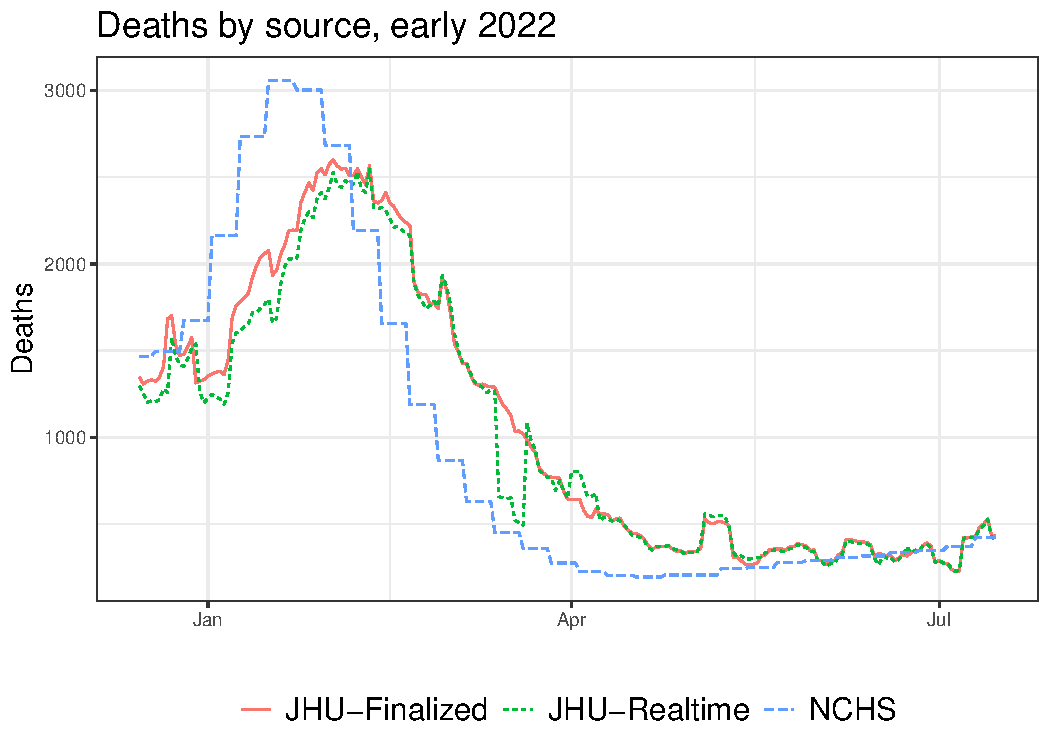
\includegraphics[width=\linewidth]{Figures/Real/death_curves.pdf}
\caption{Comparing estimates based on real-time versus finalized counts.}    
\label{fig:rt_and_final}
\end{figure}

\subsection{Hyperparameters}

We evaluate the robustness of our findings against choices of hyperparameters.
% (All results are with the finalized version of JHU deaths.) 
First, we analyze smoothed versions of the ratio estimators, where we smooth the 
numerator and denominator separately:
\begin{align*}
\hat{p}_t^{\ell,w} &= \frac{\sum_{s=t-w+1}^t Y_s}
{\sum_{s=t-w+1}^t X_{s-\ell}}, \\ 
\hat{p}_t^{\gamma,w} &= \frac{\sum_{s=t-w+1}^t Y_s}
{\sum_{s=t-w+1}^t \sum_{k=0}^d X_{s-\ell-k}\gamma_k}.
\end{align*} 
Figure \ref{fig:window} shows the results for varying window lengths $w >
0$. The results are very similar, indicating the bias does not disappear when
smoothing over a longer history.  

\begin{figure}[h!]
\centering
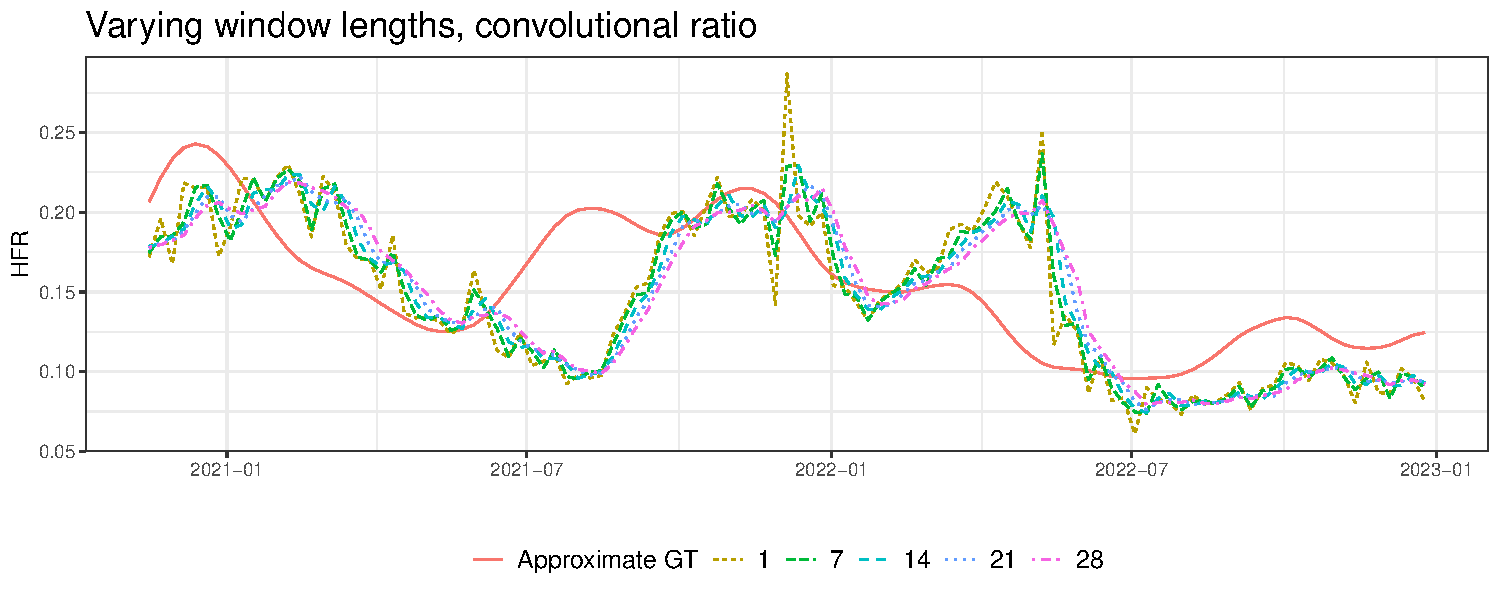
\includegraphics[width=\linewidth]{Figures/Real/window_size_conv.pdf}
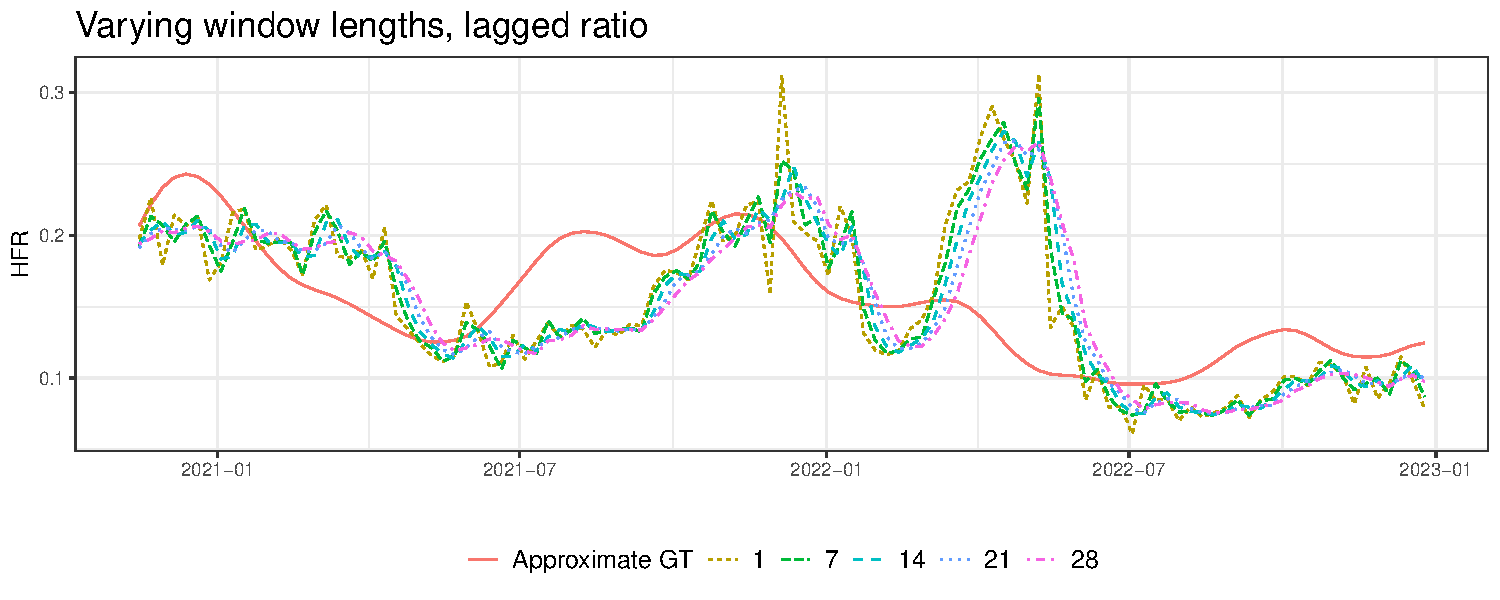
\includegraphics[width=\linewidth]{Figures/Real/window_size_lagg.pdf}
\caption{Comparing different choices of window length in post-smoothing.}
\label{fig:window}
\end{figure}

We next examine the time-to-death hyperparameters: The lag for the lagged ratio
and delay distribution for the convolutional ratio. Figure \ref{fig:lag}
displays lagged HFR estimates where the lag $\ell$ ranges from 2 to 5
weeks. Unlike the window size, changing this parameter leads to notably
different behavior. Some choices of lag are better than others; a 28-day lag,
for example, falls appropriately in winter 2021, and rises less slowly during
Delta. However, all are biased to varying degrees, most notably the huge
spurious surge in spring 2022.

\begin{figure}[p]
\centering
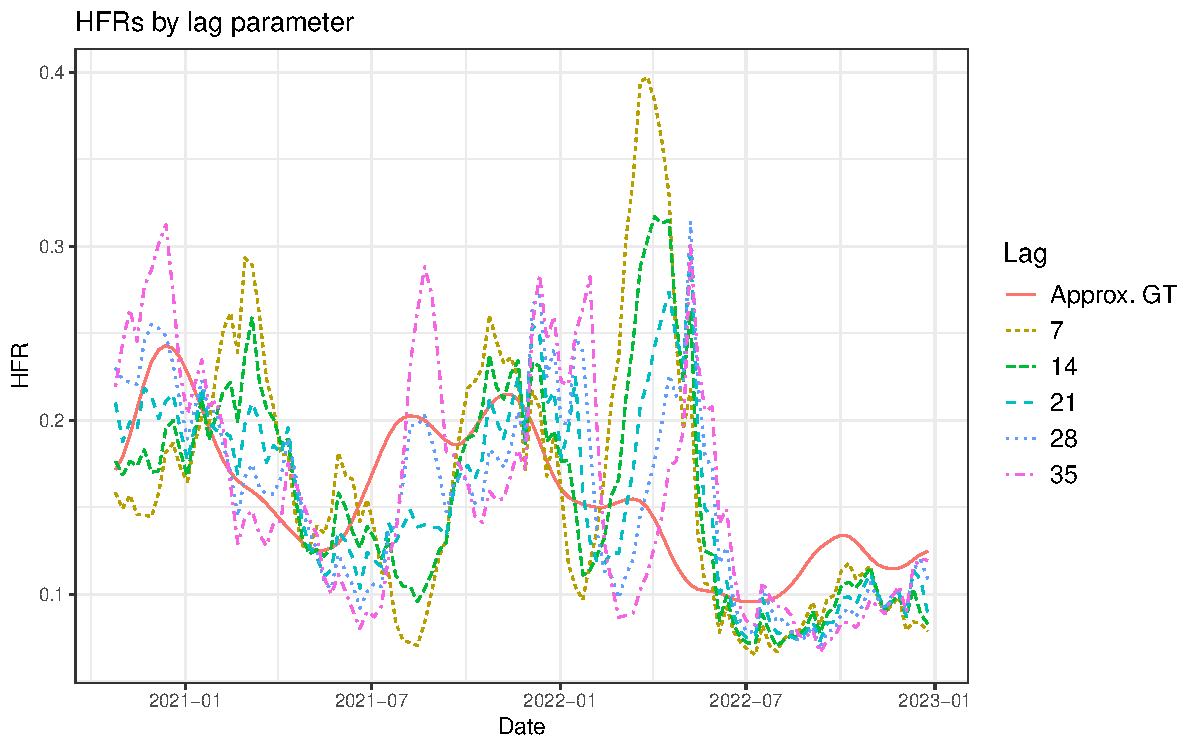
\includegraphics[width=\linewidth]{Figures/Real/hfrs_by_lag.pdf}
\caption{Comparing different choices of lag parameter in the lagged ratio.}
\label{fig:lag}

\bigskip
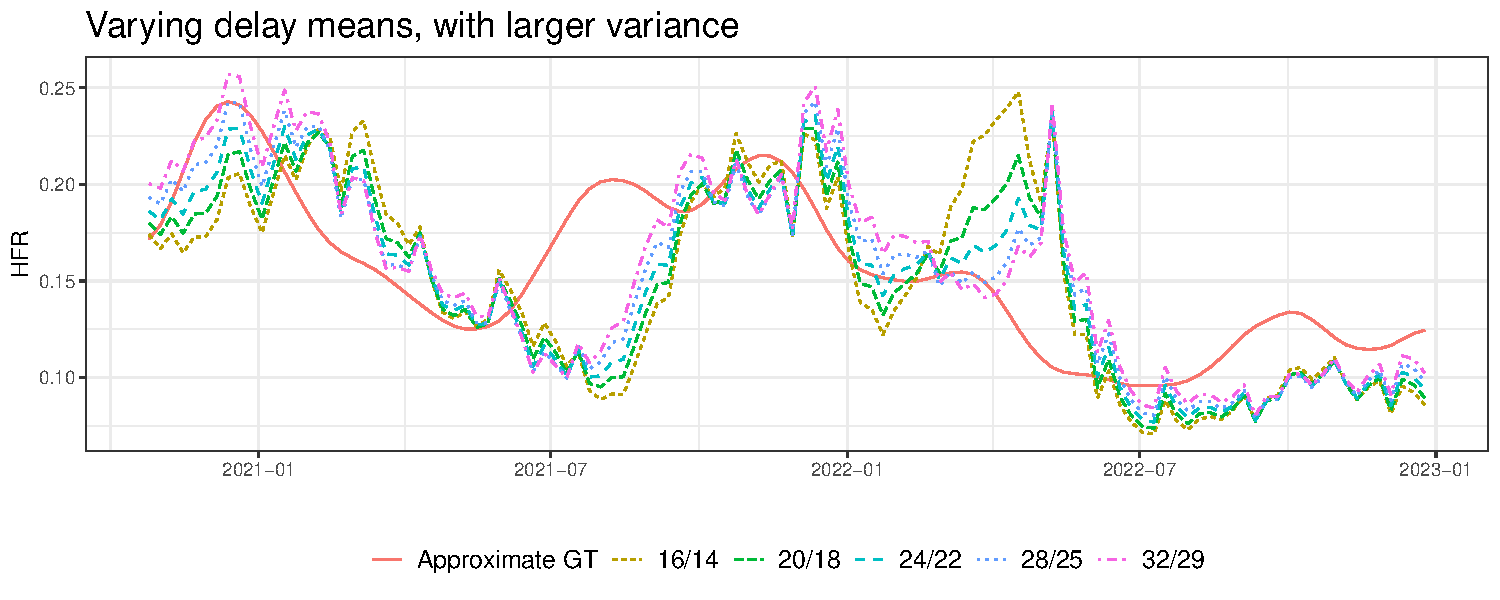
\includegraphics[width=\linewidth]{Figures/Real/hfrs_by_delay1.pdf}
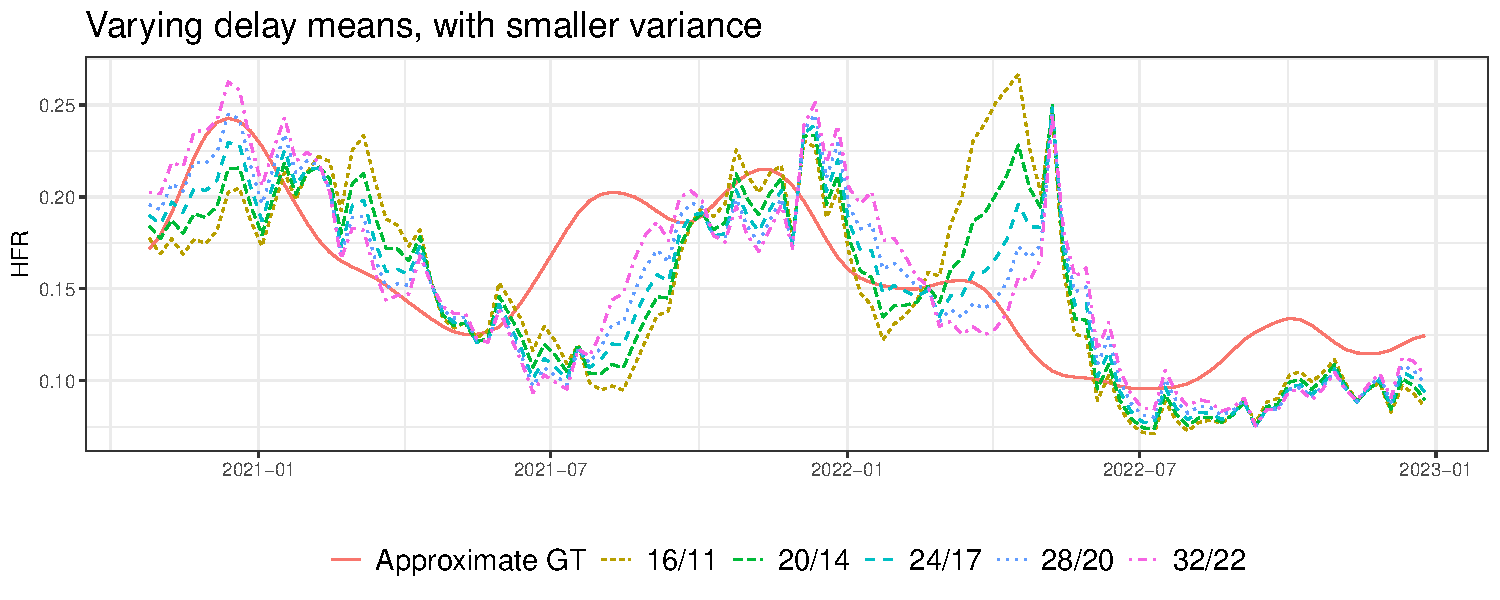
\includegraphics[width=\linewidth]{Figures/Real/hfrs_by_delay2.pdf}
\caption{Comparing different choices of delay distributions in the convolutional
  ratio. The top panel shows gamma distributions whose standard deviation is 0.9
  times the mean, versus 0.7 times the mean the bottom panel. The legend labels
  reflect the mean/standard deviation.}  
\label{fig:delays}
\end{figure}

Figure \ref{fig:delays} compares the performance of the convolutional ratio
across different choices of delay $\gamma$; we kept the discrete
gamma shape for each, but varied the mean and standard deviation. We
investigated a standard deviation equal to 90\% of the mean, and also a more
compact delay with standard deviation equal to 70\% of the mean. All
resulting HFR estimates are significantly biased. Regardless of delay
distribution, the ratios are negatively biased during the onset of Delta, and
surge after the peak of Omicron. This indicates the bulk of the error is
fundamental to the estimator, and cannot be attributed to model
misspecification.     

% Comparing to the approximate ground truth HFRs from NHCS, performance improved 
% slightly with a longer delay distribution than the purported mean of 20 
% days. Its mean absolute error was 0.031, whereas the delay distribution with 
% mean 28 and standard deviation 25 had a MAE of 0.27. Nevertheless, this 
% difference is relatively small, with the alternative delay distribution still 
% showing similar bias.  

\subsection{State-level results}

We repeat our analysis the six large US states, finding similar trends. The NHCS
survey was conducted on a subset of hospitals meant to represent the US at
large, so for the state-level approximate ground truth, we therefore use the
forward-looking lagged ratio computed using NCHS deaths, as discussed above.
Figure \ref{fig:state-level} compares this rough ground truth to the real-time 
convolutional and lagged ratios. For each state, we select the lag for the
approximate ground truth curve to maximize cross-correlation between
hospitalizations and NCHS deaths, and the lag in the real-time lagged ratio to
maximize cross-correlation between hospitalizations and JHU deaths. We then use
a discrete gamma distribution with mean equal to the latter lag, and standard
deviation 90\% of its mean, for the convolutional ratio.

\begin{figure}[htbp]
\centering
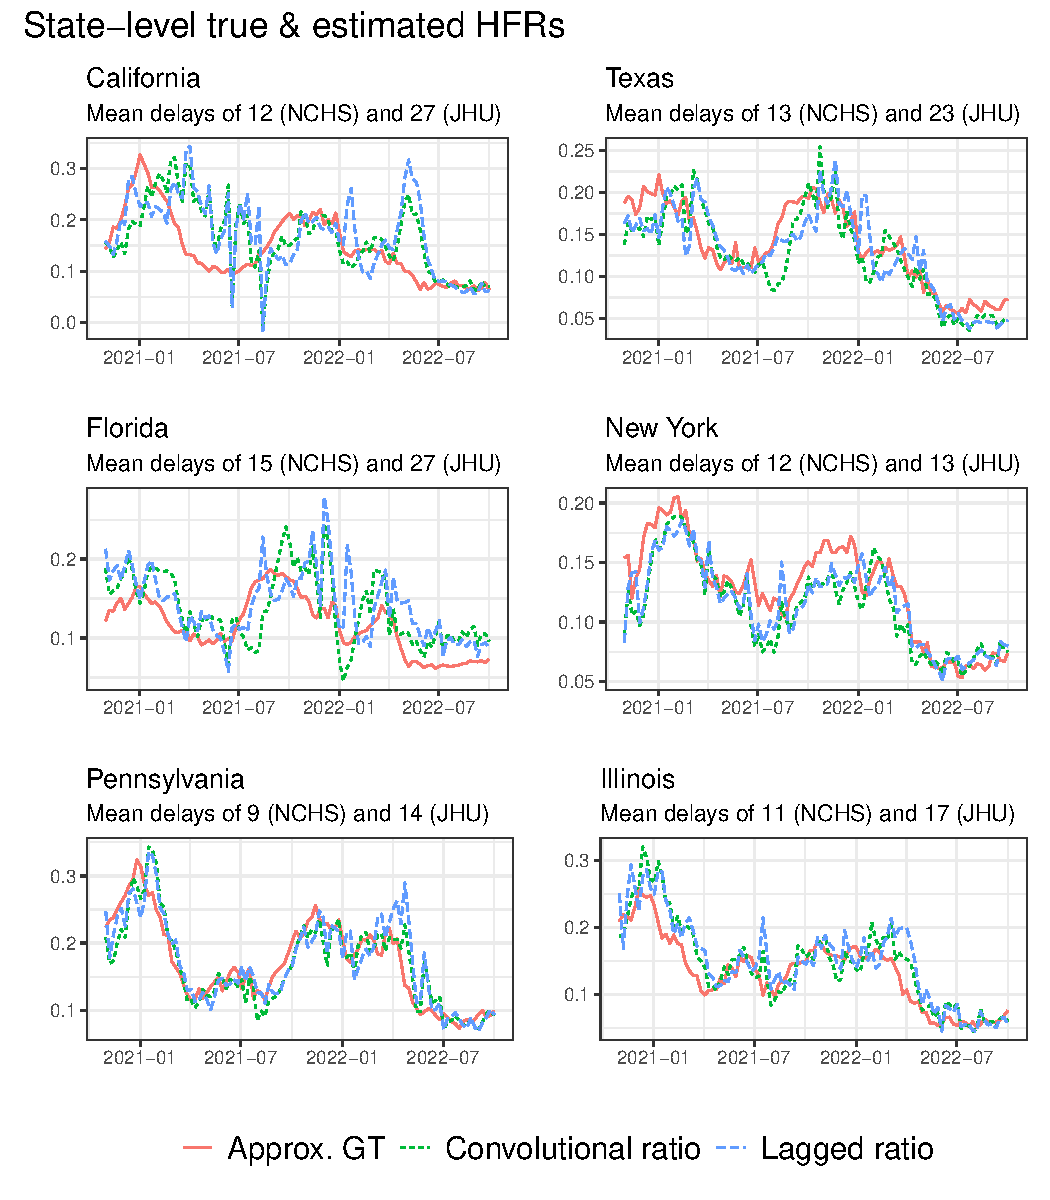
\includegraphics[width=\linewidth]{Figures/Real/state_level_hfrs.pdf}
\caption{Comparing ratio estimates for individual US states.} 
\label{fig:state-level}
 \end{figure}

Several states display similar biases to the US as whole (Figure
\ref{fig:basic_est_vs_gt_figs}). Estimates in California, Texas, and Florida are 
all slow to detect the uptick in HFR during Delta; they also spike during
Omicron in California, and to a lesser extent Florida. Note these states are the
ones with the largest cross-correlation optimal lags, an estimate of the average 
time-to-death. In contrast, New York, Pensylvania, and Illinois have mean delays
of at most 17. Their HFR estimates are still biased, but overall less so. This
once again emphasizes the role of the delay in bias. The takeaway: fatality
ratios are generally less trustworthy in states that take longer to report
deaths.         

% \section{Miscellaneous results}\label{apx:misc}

% \subsection{Alternative lag on simulation}
% \begin{figure}
%     \centering
%     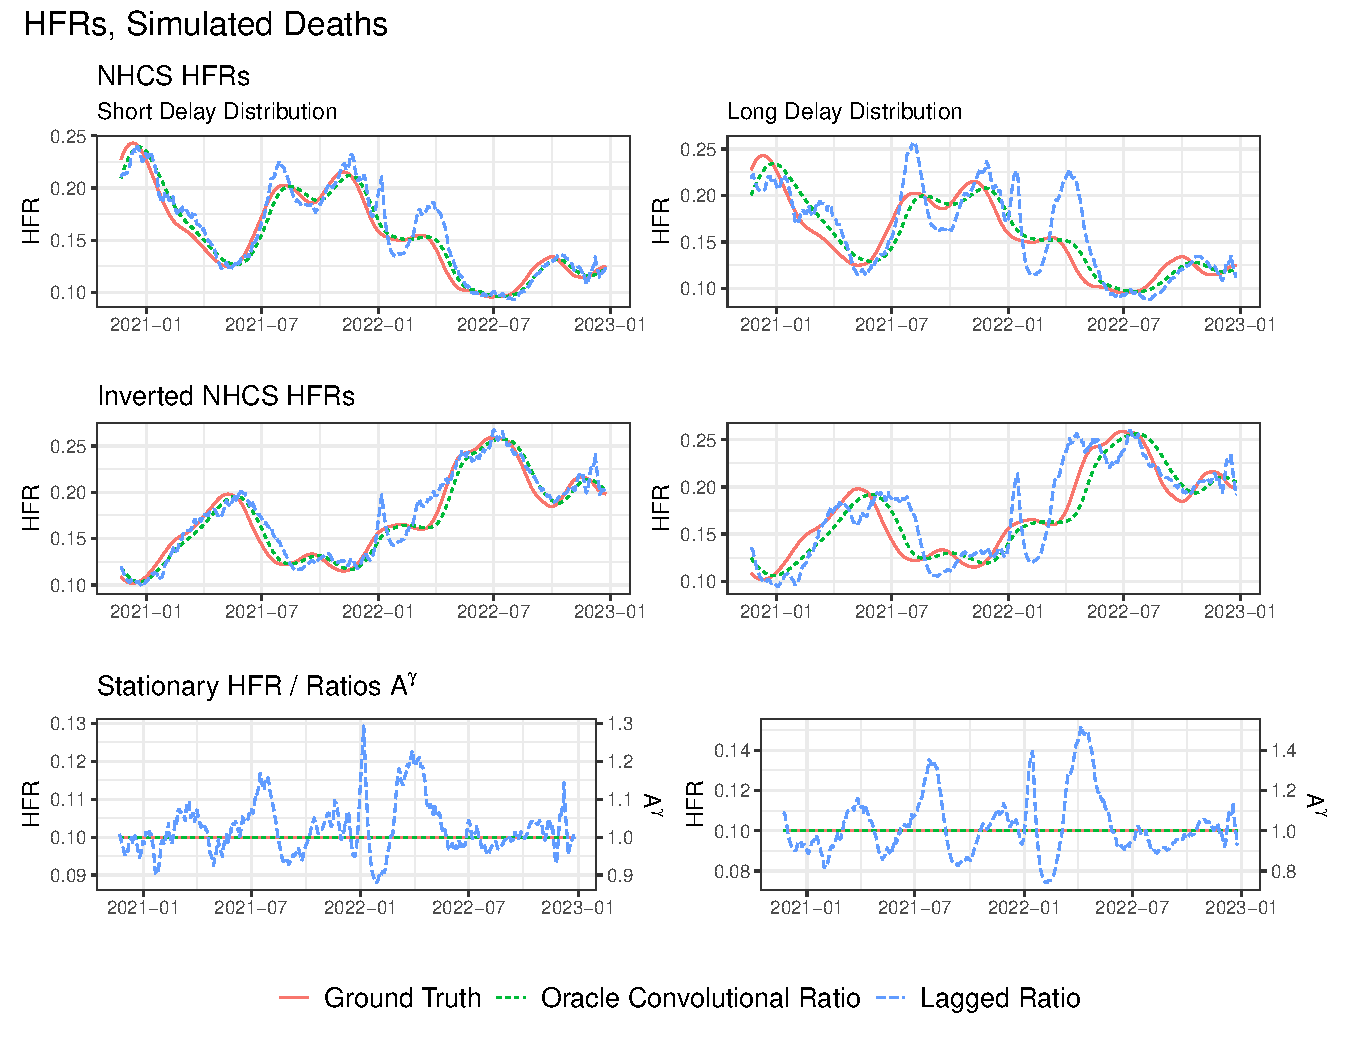
\includegraphics[width=\linewidth]{Figures/Simulated/simulated_results_delay_mean.pdf} 
%     \caption{Lag chosen as mean of delay distribution. Same simulated data as
%     Section~\ref{sec:results_sim}.} 
%     \label{fig:sims_mean_lag}
% \end{figure}

% Figure \ref{fig:sims_mean_lag} presents the simulation results from
% Section~\ref{sec:results_sim} when the lag is the mean of the delay
% distribution. It clearly indicates the lagged ratio is not markedly better
% under this lag. This is in step with Figure \ref{fig:lag}, which demonstrated
% that its performance on real data are robust to choice of lag. 

\end{document}
